\documentclass[12pt,a4paper]{article}
\usepackage[utf8x]{inputenc}
\usepackage{ucs}
\usepackage[MeX]{polski}
\usepackage{fancyhdr}
\usepackage{amsmath}
\usepackage{amsfonts}
\usepackage{amssymb}
\pagestyle{plain}
\usepackage{enumerate}
\usepackage{listings}
\usepackage{graphicx}
%\usepackage{subfig}
\usepackage{caption}
\usepackage{float}
\usepackage{tabularx}
\usepackage{nameref}
\usepackage{subcaption}

%Dokumentacja techniczna projektu Rękawica Sensoryczna 2017
\usepackage{graphicx}
\usepackage{hyperref}


\renewcommand{\maketitle}{\begin{titlepage}

\begin{center}


\LARGE\centering Dokumentacja techniczna projektu Rękawica Sensoryczna\\
\large\centering Projekt realizowany w ramach kursu Roboty Mobilne 1 na Politechnice Wrocławskiej\\
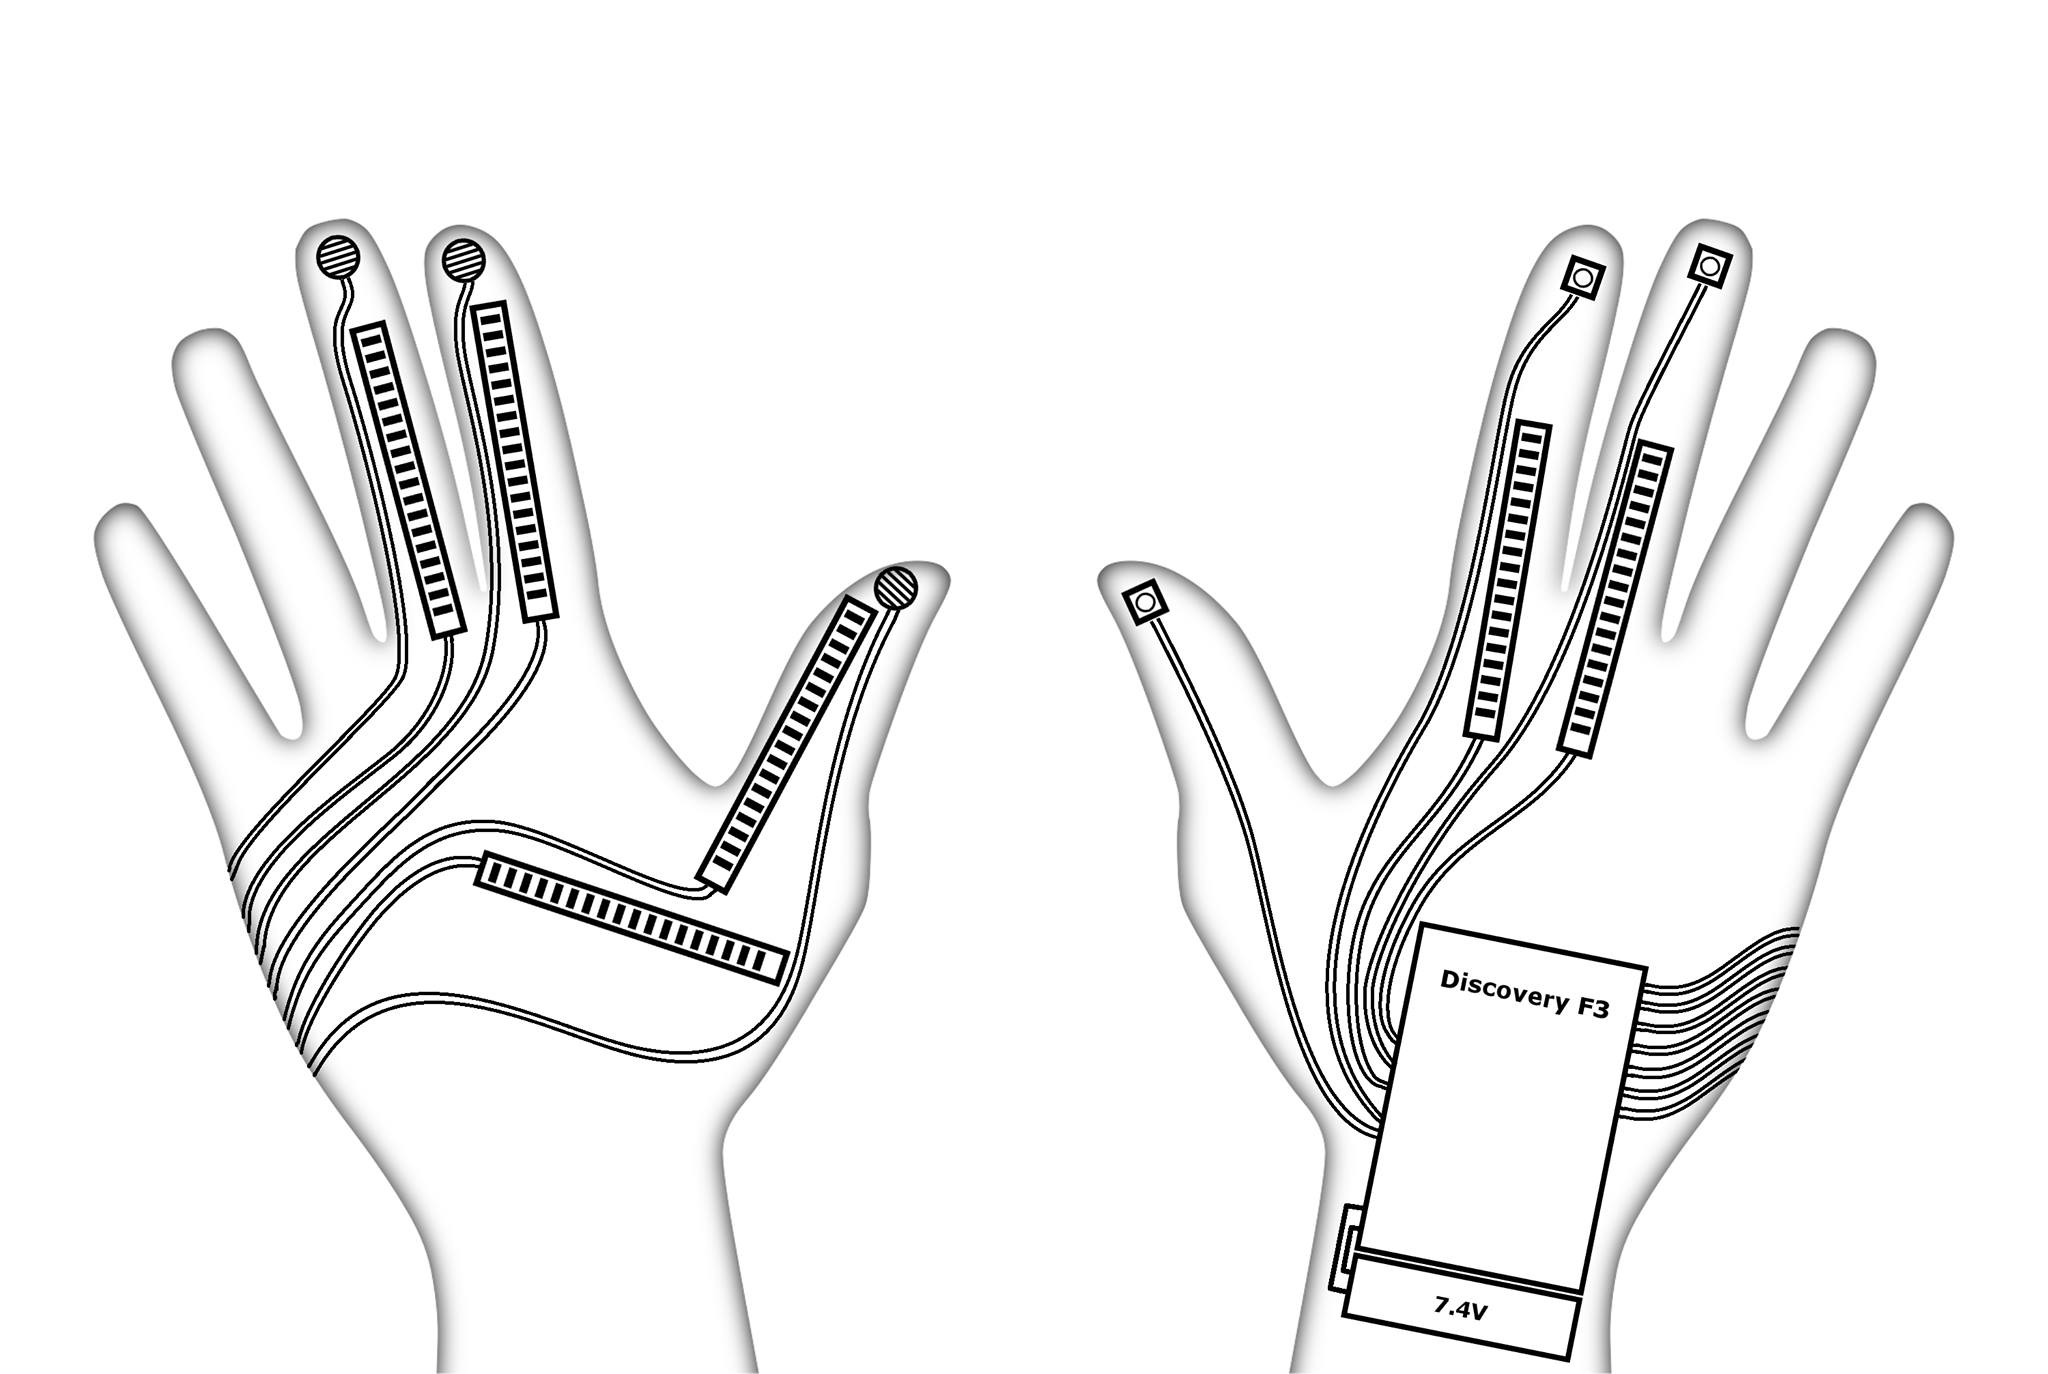
\includegraphics[width=0.7\textwidth]{images/rekawica_old.jpg}
\vspace*{2cm}
\normalsize\flushleft\textbf{Temat Projektu:} Rękawica sensoryczna\\
\textbf{Autorzy:} Krzysztof Dąbek 218549, Dymitr Choroszczak 218627,\\Anna Postawka 218556\\
\textbf{Kierunek:} Automatyka i Robotyka\\
\textbf{Specjalność:} Robotyka (ARR)\\
\textbf{Prowadzący:} dr inż. Andrzej Wołczowski\\
\textbf{Kurs:} Roboty Mobilne 1\\
\textbf{Termin zajęć:} pn TN 11:15, śr TN 14:30\\
\vspace{5 mm}



\vspace*{3.5cm}
\centering\textsc{\today}\\

\end{center}
\end{titlepage}
\newpage
}
\begin{document}
\maketitle
\tableofcontents
\newpage


\section{Główne założenia projektowe: }\normalsize
\begin{itemize}
\item Stworzenie rękawicy z czujnikami ugięcia w trzech palcach oraz czujnikami nacisku na opuszkach
\item Zamontowanie na opuszkach LEDów (np. RGB) wizualizujących odczyty z czujników nacisku
\item Wykorzystanie płytki STM32F3Discovery do przetwarzania danych
\item Użycie akcelerometru zawartego na płytce do określenia położenia dłoni względem pionu (wektora przyśpieszenia grawitacyjnego)
\item Bezprzewodowe przesyłanie danych do komputera za pomocą modułu Bluetooth HC-06
\item Przewodowe przesyłanie danych do komputera za pomocą interfejsu USB
\item Zewnętrzne zasilanie z akumulatora
\item Uproszczony model dłoni w wizualizacji 3D
\end{itemize}

\section{Opis czujników}
\begin{itemize}
\item Na opuszkach palców zamontowano \textbf{czujniki nacisku FSR-400 Short od Interlink Electronics}. Spadek rezystancji przy przyłożonej sile pozwala zmierzyć siłę nacisku [rys. \ref{fig:wykresy_fsr-400}].
\item Do wykrycia zgięcia stawów międzypaliczkowych i śródręczno-paliczkowych oraz stawów kciuka zastosowano \textbf{czujniki ugięcia -- Flex Sensory 2.2" firmy Spectra Symbol}. Zgięcie tych sensorów powoduje wzrost rezystancji.
\item \textbf{Akcelerometr LSM303DLHC}, znajdujący się na płytce Discovery został użyty do określenia orientacji rękawicy względem wektora grawitacji.
\end{itemize}
\subsection{Dane czujnika nacisku}
\begin{itemize}
\item Średnica powierzchni czynnej: 5 mm
\item Zakres pomiarowy nacisku: 0.2 - 20 N
\item Zakres rezystancji: 150 Ohm - 10 MOhm
\item Rezystor pomiarowy do dzielnika: 3 kOhm
\end{itemize}
\subsection{Dane czujnika ugięcia}
\begin{itemize}
\item Długość powierzchni czynnej: 55.37 mm
\item Zakres rezystancji: 25 kOhm - 125 kOhm
\item Rezystor pomiarowy do dzielnika: 62 kOhm
\end{itemize}
\subsection{Dane z akcelerometru}
\begin{itemize}
\item Protokół komunikacyjny: $I^2C$
\item Ilość osi: 3
\item Maksymalne przeciążenie: 16g
\item Dokładność pomiaru: 16 bitów 
\end{itemize}
%\subsection{Parametry}

\begin{figure}[!htb]
\centering
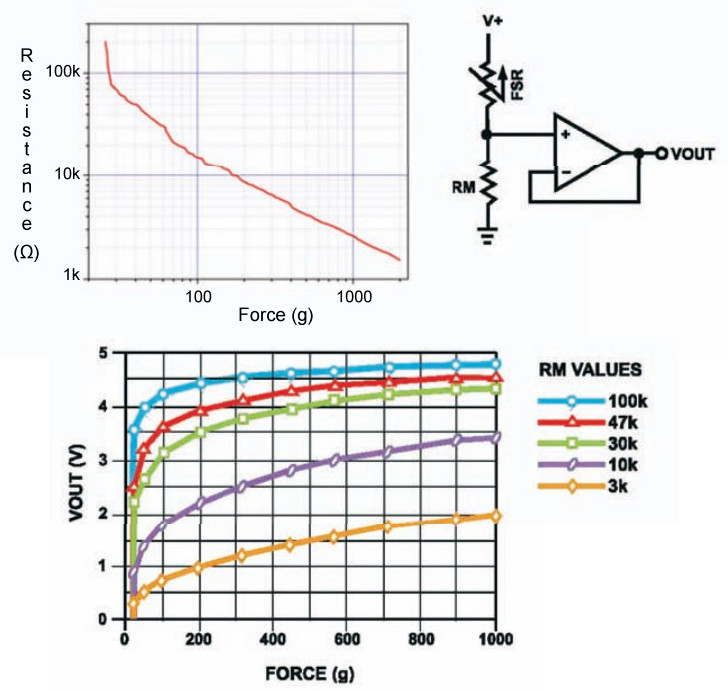
\includegraphics[width=0.8\textwidth]{images/fsr-400.jpg}
\caption{Układ pomiarowy oraz wykresy zależności napięć i rezystancji od przyłożonej siły dla czujnika FSR-400}
\label{fig:wykresy_fsr-400}
\end{figure}

\begin{table}[!htb]
\centering
\begin{tabularx}
{\textwidth}{ |X|X| }
\hline
Zakres & 0,2--20 N \\
\hline
Masa & 0,15 g \\ 
\hline
Wymiary zewnętrzne & 7,6 x 7,6 x 0,4 mm \\
\hline
\end{tabularx}
\caption{Czujnik siły nacisku FSR-400}
\end{table}


\begin{table}[!htb]
\centering
\begin{tabularx}
{\textwidth}{ |X|X| }
\hline
Min. wartość rezystancji & 25 k$\Omega$ \\
\hline
Zakres rezystancji podczas zginania & 45--125 k$\Omega$ \\
\hline
Dł. całkowita & 73,66 mm \\
\hline
Dł. użyteczna czujnika & 55,37 mm \\ 
\hline
Szerokość & 6,35 mm \\
\hline
\end{tabularx}
\caption{Czujnik ugięcia Flex Sensor 2.2"}
\end{table}


\begin{table}[!htb]
\centering
\begin{tabularx}
{\textwidth}{ |X|X| }
\hline
Napięcie pracy & 2,2--3,6 V \\
\hline
Interfejs komunikacyjny & I2C \\
\hline
Rozdzielczość & 16 bitów \\
\hline
Regulowany zakres akcelerometru &  $\pm$2g, $\pm$4g, $\pm$8g, $\pm$16g \\ 
\hline
Zakres magnetometru &  od $\pm$1,3 do $\pm$8,1 gauss \\ 
\hline
Wymiary płytki & 37 x 15 mm \\
\hline
\end{tabularx}
\caption{LSM303DLHC -- 3-osiowy akcelerometr i magnetometr I2C}
\end{table}

\section{Elementy składowe projektu}
Rękawica sensoryczna zbiera dane z trzech palców prawej ręki. Czujniki ugięcia przyszyto na zewnętrznej stronie dłoni [rys. \ref{fig:gotowa}].
 Przetestowano kilka ustawień czujników i takie zdaje się najlepiej spełniać założenia, czyli poprawnie odczytywać zgięcia konkretnych stawów palców, nie ograniczając przy tym ruchów dłoni. Czujniki nacisku przymocowano na opuszkach [rys. \ref{fig:gotowa2}]. Zostały one przyklejone klejem błyskawicznym. Przymocowano również na wierzchu dłoni 2 listwy żeńskie do wpięcia płytki Discovery F3, aby móc pobierać dane z akcelerometru i wykrywać obrót ręki [rys. \ref{fig:gotowa}].
 
\begin{figure}[!htb]
\centering
\begin{subfigure}{.5\textwidth}
	\centering
	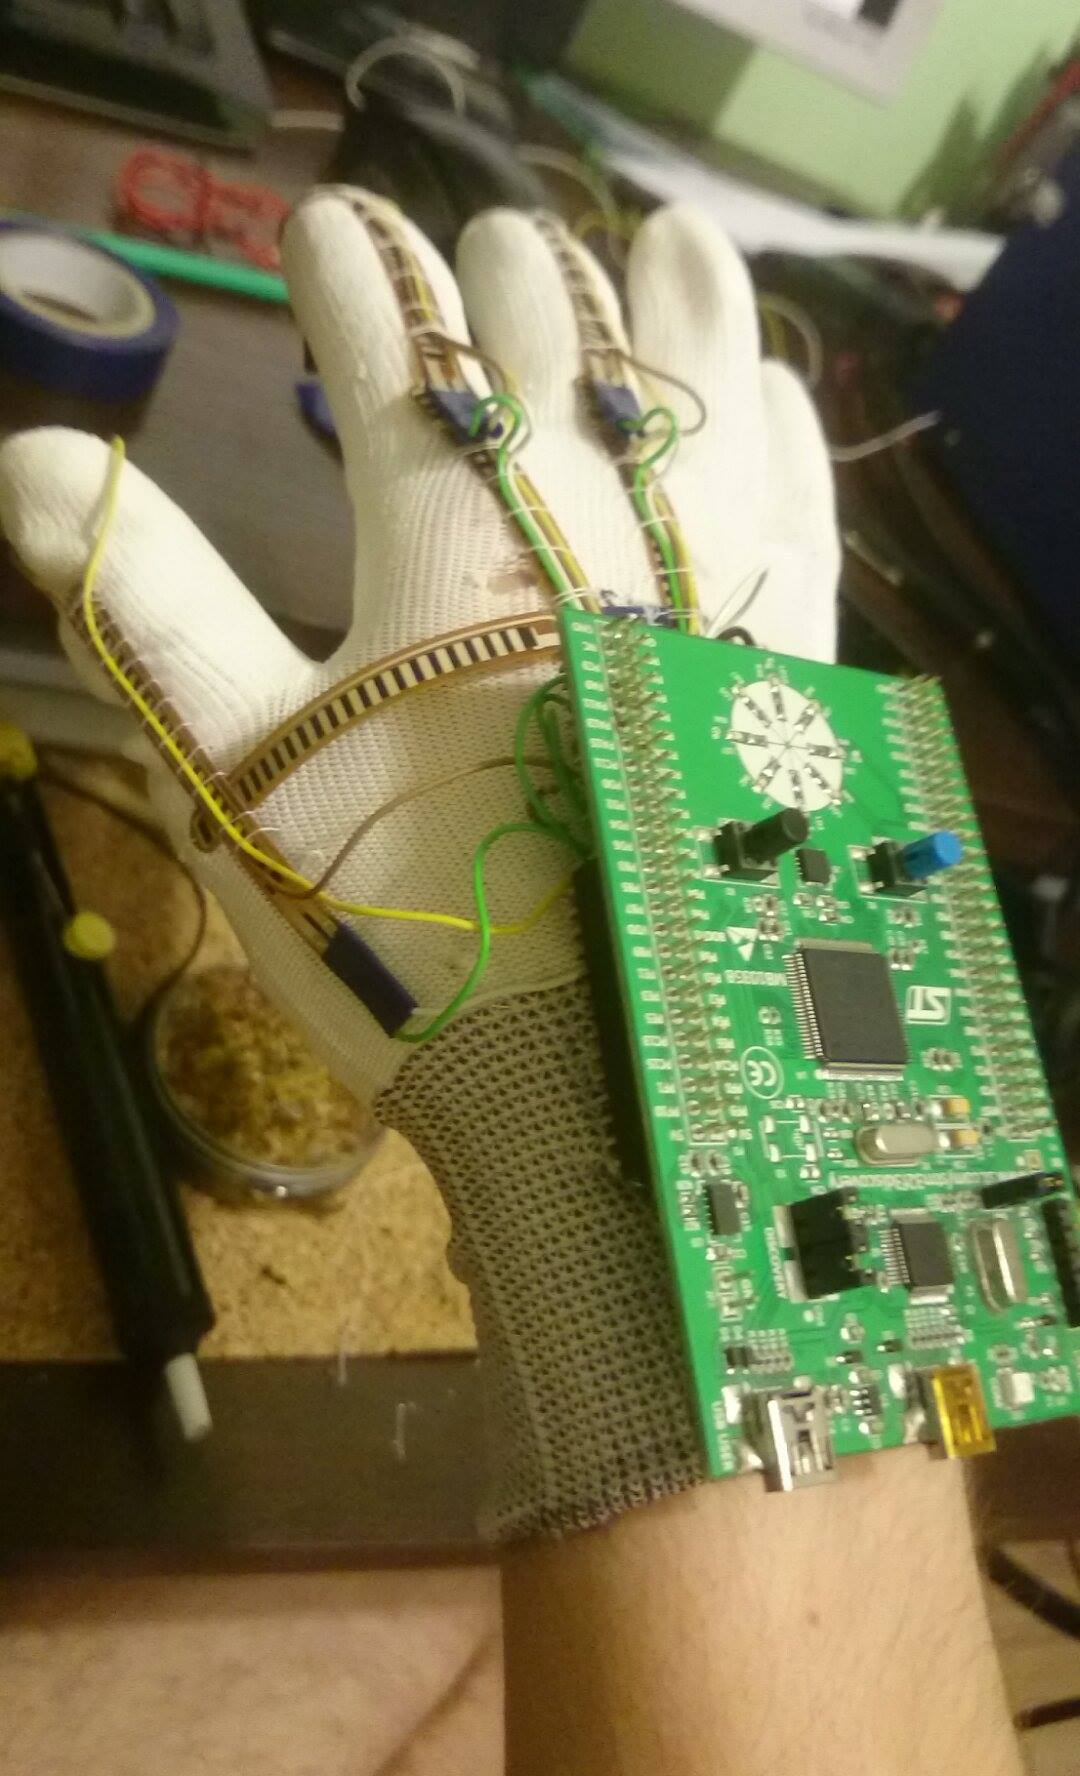
\includegraphics[width=.9\textwidth]{images/gotowa.jpg}
	\caption{Zewnętrzna część dłoni}
	\label{fig:gotowa}
\end{subfigure}%
\begin{subfigure}{.5\textwidth}
	\centering
	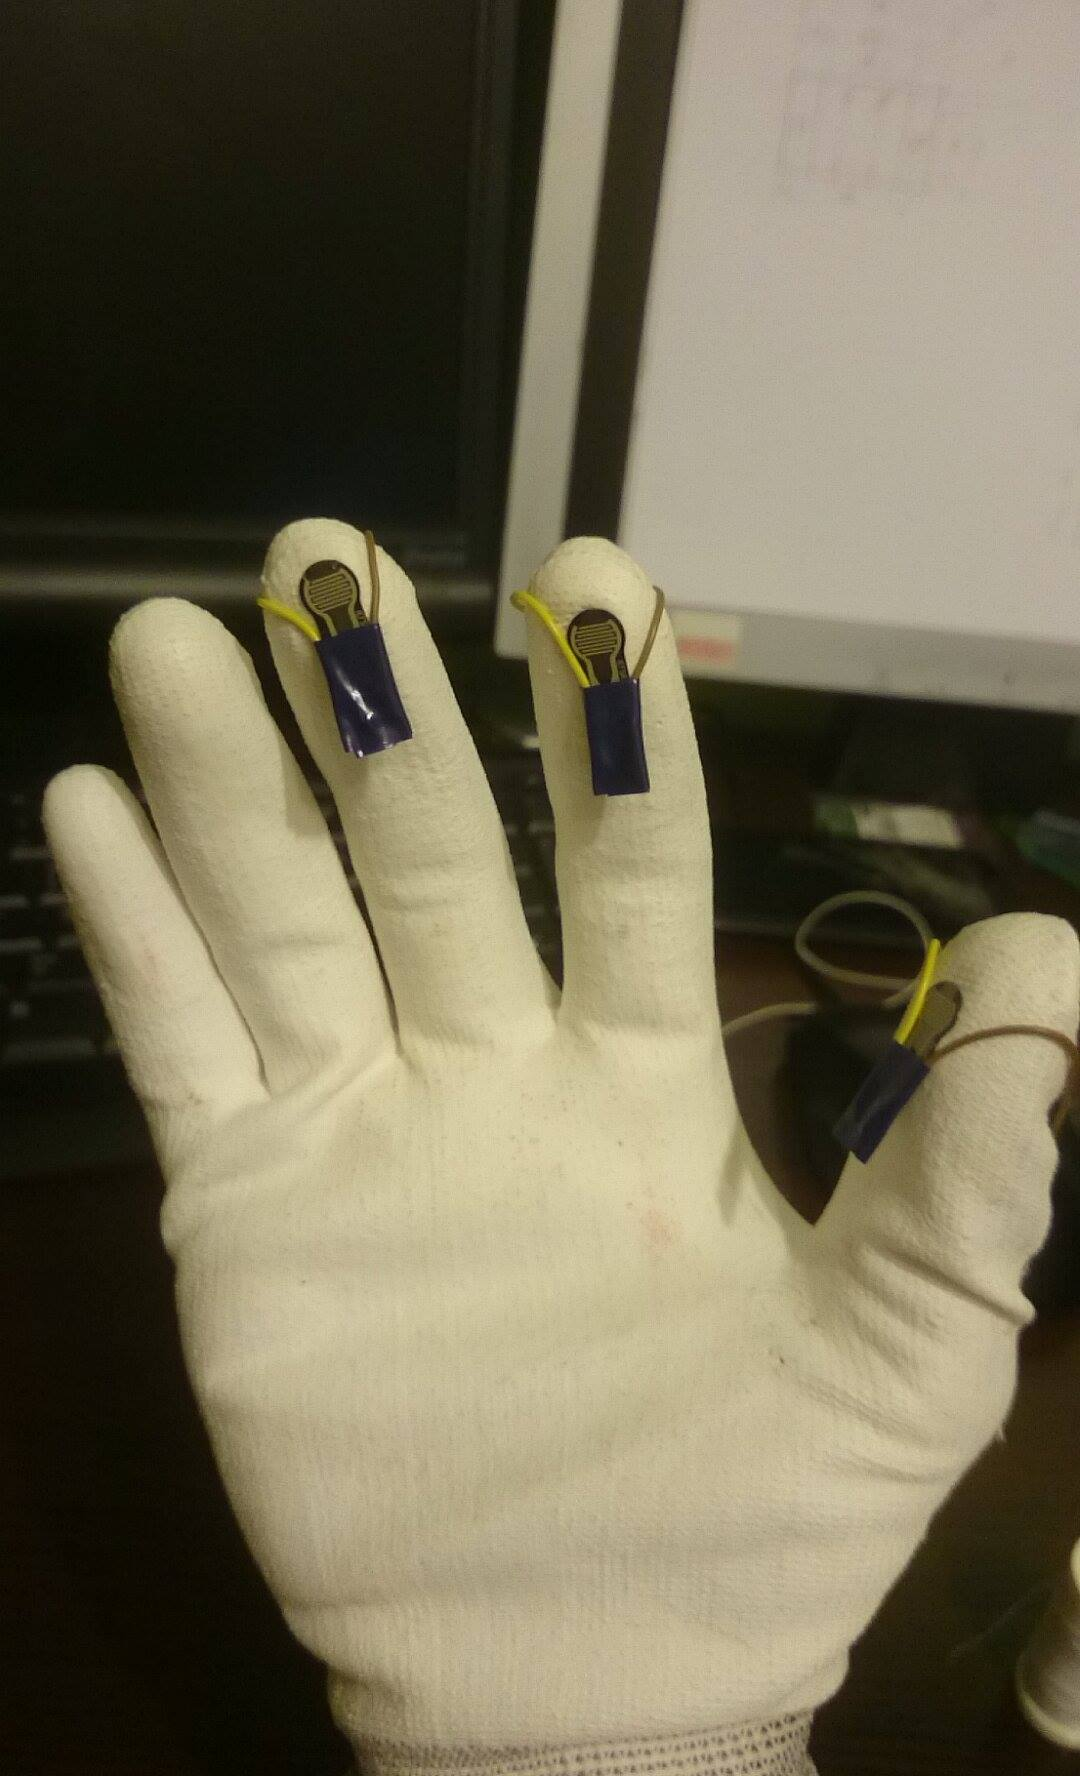
\includegraphics[width=.9\textwidth]{images/gotowa2.jpg}
	\caption{Wewnętrzna część dłoni}
	\label{fig:gotowa2}
\end{subfigure}
\caption{Gotowa rękawica}
\label{fig:gotowa_rekawica}
\end{figure}

\subsection{Połączenie z komputerem}
Płytka STM32F3DISCOVERY potrafi połączyć się z komputerem za pomocą interfejsu USB i UART. Zrezygnowano z połączenia za pomocą Bluetooth ze względu na zbyt małą szybkość przesyłania oraz niepoprawne funkcjonowanie modułu Bluetooth komputera.

\subsection{Odczyt danych z czujników}
\subsubsection{Tensometry} \label{tensometry}
Dane z czujników są odczytywane za pomocą przetwornika ADC oraz przy użyciu DMA (Direct Memory Access), co pozwala na bezpośrednie przekierowanie danych z czujników do odpowiednich zmiennych, bez wywoływania dodatkowej funkcji zwracającej wynik pomiaru.
\subsubsection{Czujniki nacisku}
Obsługa taka sama jak w: \nameref{tensometry}.
\subsubsection{Akcelerometr}
Z akcelerometrem komunikacja następuje po interfejsie I2C.



\subsection{Wizualizacja dłoni}
Aplikacja pozwala na wizualizację modelu ręki na podstawie odczytów z czujników. Powstała we frameworku Qt. Aktualny interfejs graficzny wyświetla uproszczony model dłoni [rys. \ref{fig:wds}].
\subsection{Pomiar parametrów w czasie rzeczywistym}
Projekt umożliwia podglądanie następujących parametrów w programie STMStudio:
\begin{itemize}
\item Przetwarzanie na wolty
\item Przetwarzanie na $m/s^2$
\item Przetwarzanie na nastawy przegubów
\item Przetwarzanie na kąty RPY
\end{itemize}
Powyższe wartości są filtrowane na bieżąco przez filtr dolnoprzepustowy ze zmiennym parametrem $\beta$.
\begin{equation}
y[n] - \beta y[n-1] = (1-\beta)x[n]
\end{equation}


\begin{figure}[htb!]
\centering
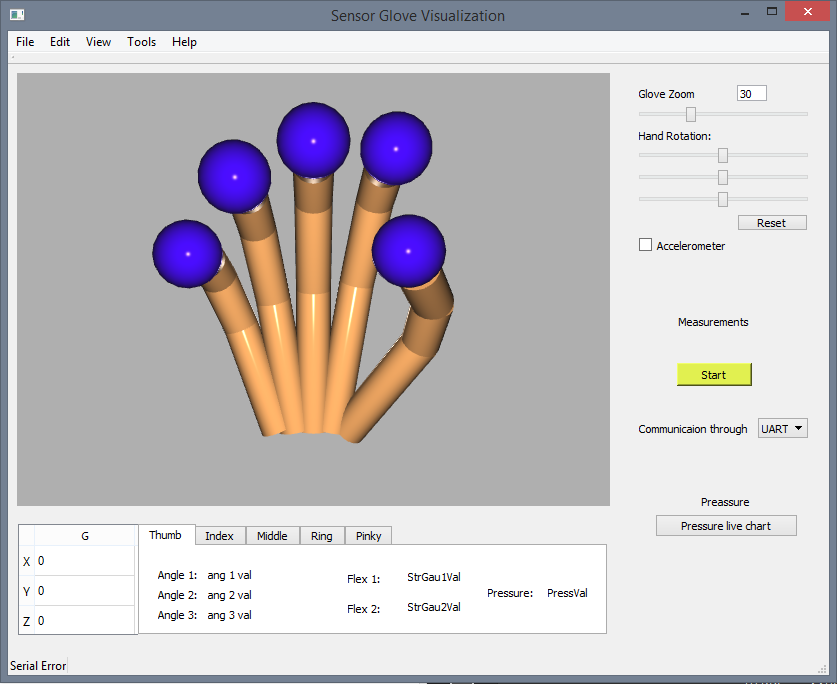
\includegraphics[width=0.8\textwidth]{images/aktualnyinterfejsgraficzny.png}
\caption{Aktualny interfejs graficzny}
\label{fig:wds}
\end{figure}

\begin{figure}[htb!]
\centering
\begin{subfigure}{.5\textwidth}
	\centering
	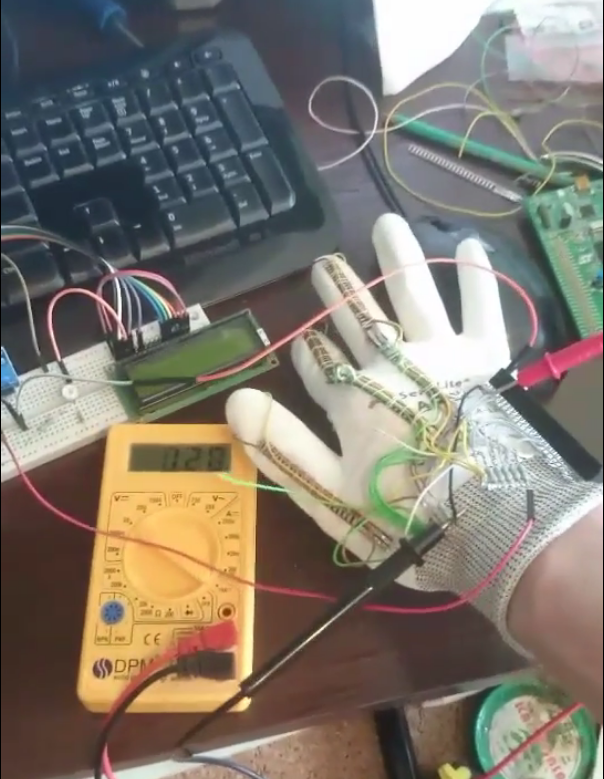
\includegraphics[width=.9\textwidth]{images/nacisk.png}
	\caption{Testowanie czujników nacisku}
	\label{fig:nacisk}
\end{subfigure}%
\begin{subfigure}{.5\textwidth}
	\centering
	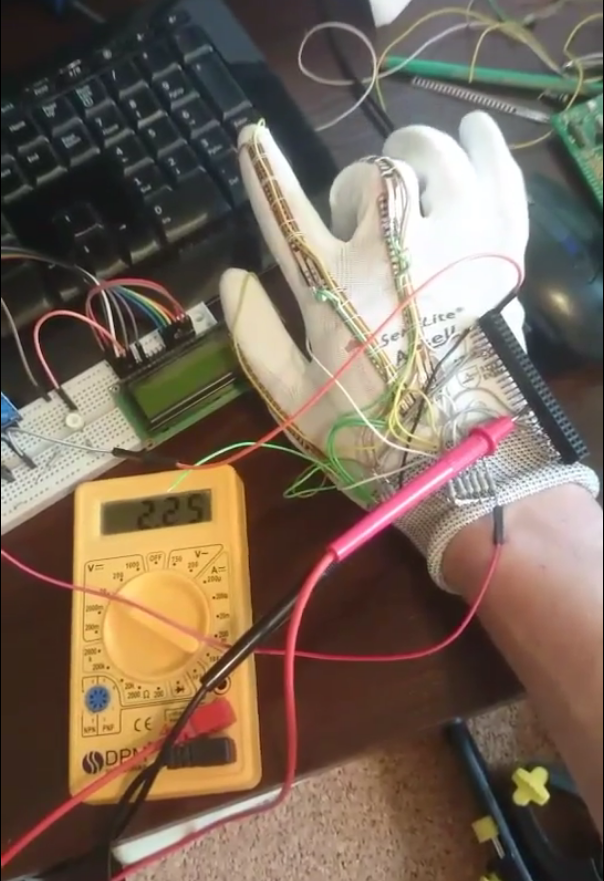
\includegraphics[width=.9\textwidth]{images/ugiecie.png}
	\caption{Testowanie czujników ugięcia}
	\label{fig:ugiecie}
\end{subfigure}
\caption{Testy}
\label{fig:testy}
\end{figure}

\newpage
\section{Badania z wykorzystaniem rękawicy}
Rękawica sensoryczna pozwala na zbieranie pomiarów i próbę jak najdokładniejszego wykrycia konkretnych gestów ludzkiej dłoni na podstawie odczytów z czujników. Takie badania mogą być wykorzystywane m.in. przy rozwoju protez biomedycznych. Takie gesty mogą posłużyć sterowaniu robotem lub systemem automatyki (np. budynkowej). Przyporządkowanie gestu do wykonywanej czynności daje możliwość kontroli systemu.\\
Wykrywanie gestów sprowadza się do ustawienia odpowiednich progów na niektórych czujnikach ugięcia i nacisku, po których przekroczeniu sygnalizuje się wykrycie gestu.\\

\subsection{Dane pomiarowe}
Zbadano poprawność pozyskiwania i wysyłania danych pomiarowych za pomocą terminala (Realterm) oraz programu STMStudio. Wyniki przedstawiono na rysunkach (\ref{fig:term}, \ref{fig:stmstudio}).\\
\begin{figure}
\centering
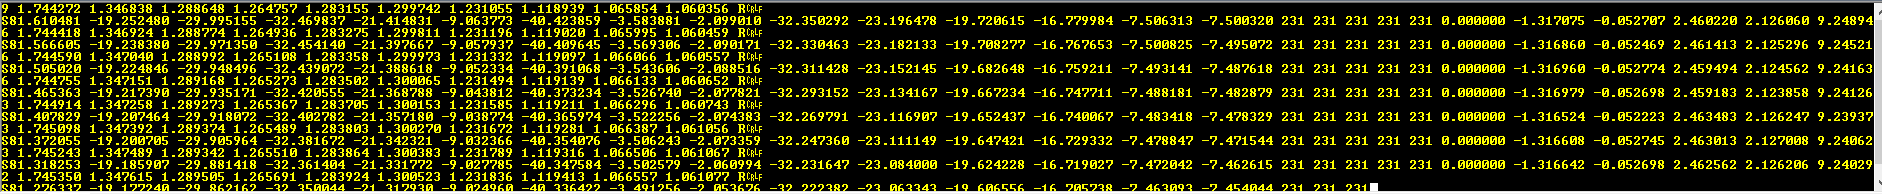
\includegraphics[width=\textwidth]{./images/terminal.png}
\caption{Wysyłane dane wyświetlone na terminalu \label{fig:term}}
\end{figure}
\begin{figure}
\centering
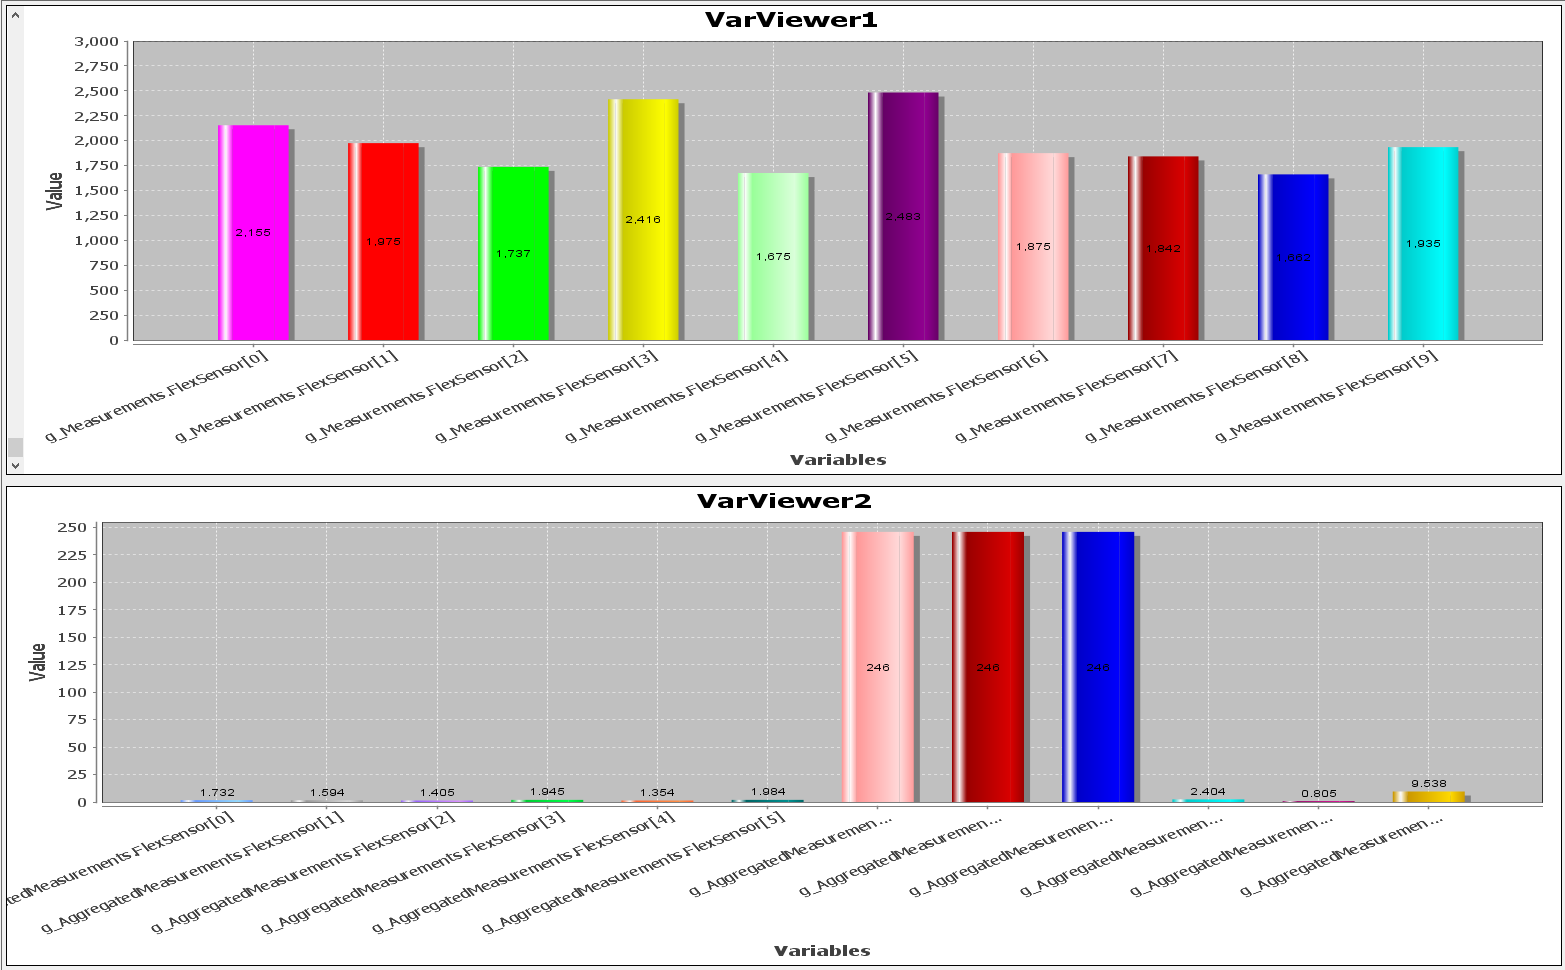
\includegraphics[width=\textwidth]{./images/stmstudio.png}
\caption{Pobierane dane wyświetlone w STMStudio\label{fig:stmstudio}}
\end{figure}

\subsection{Przykładowe gesty}
Badane gesty zostały przedstawione na rysunkach (\ref{fig:Fist}, \ref{fig:Palm}, \ref{fig:OK}, \ref{fig:Peace}, \ref{fig:Point}).
\begin{figure}[!htb]
\centering
    \begin{subfigure}{.5\textwidth}
    \centering
      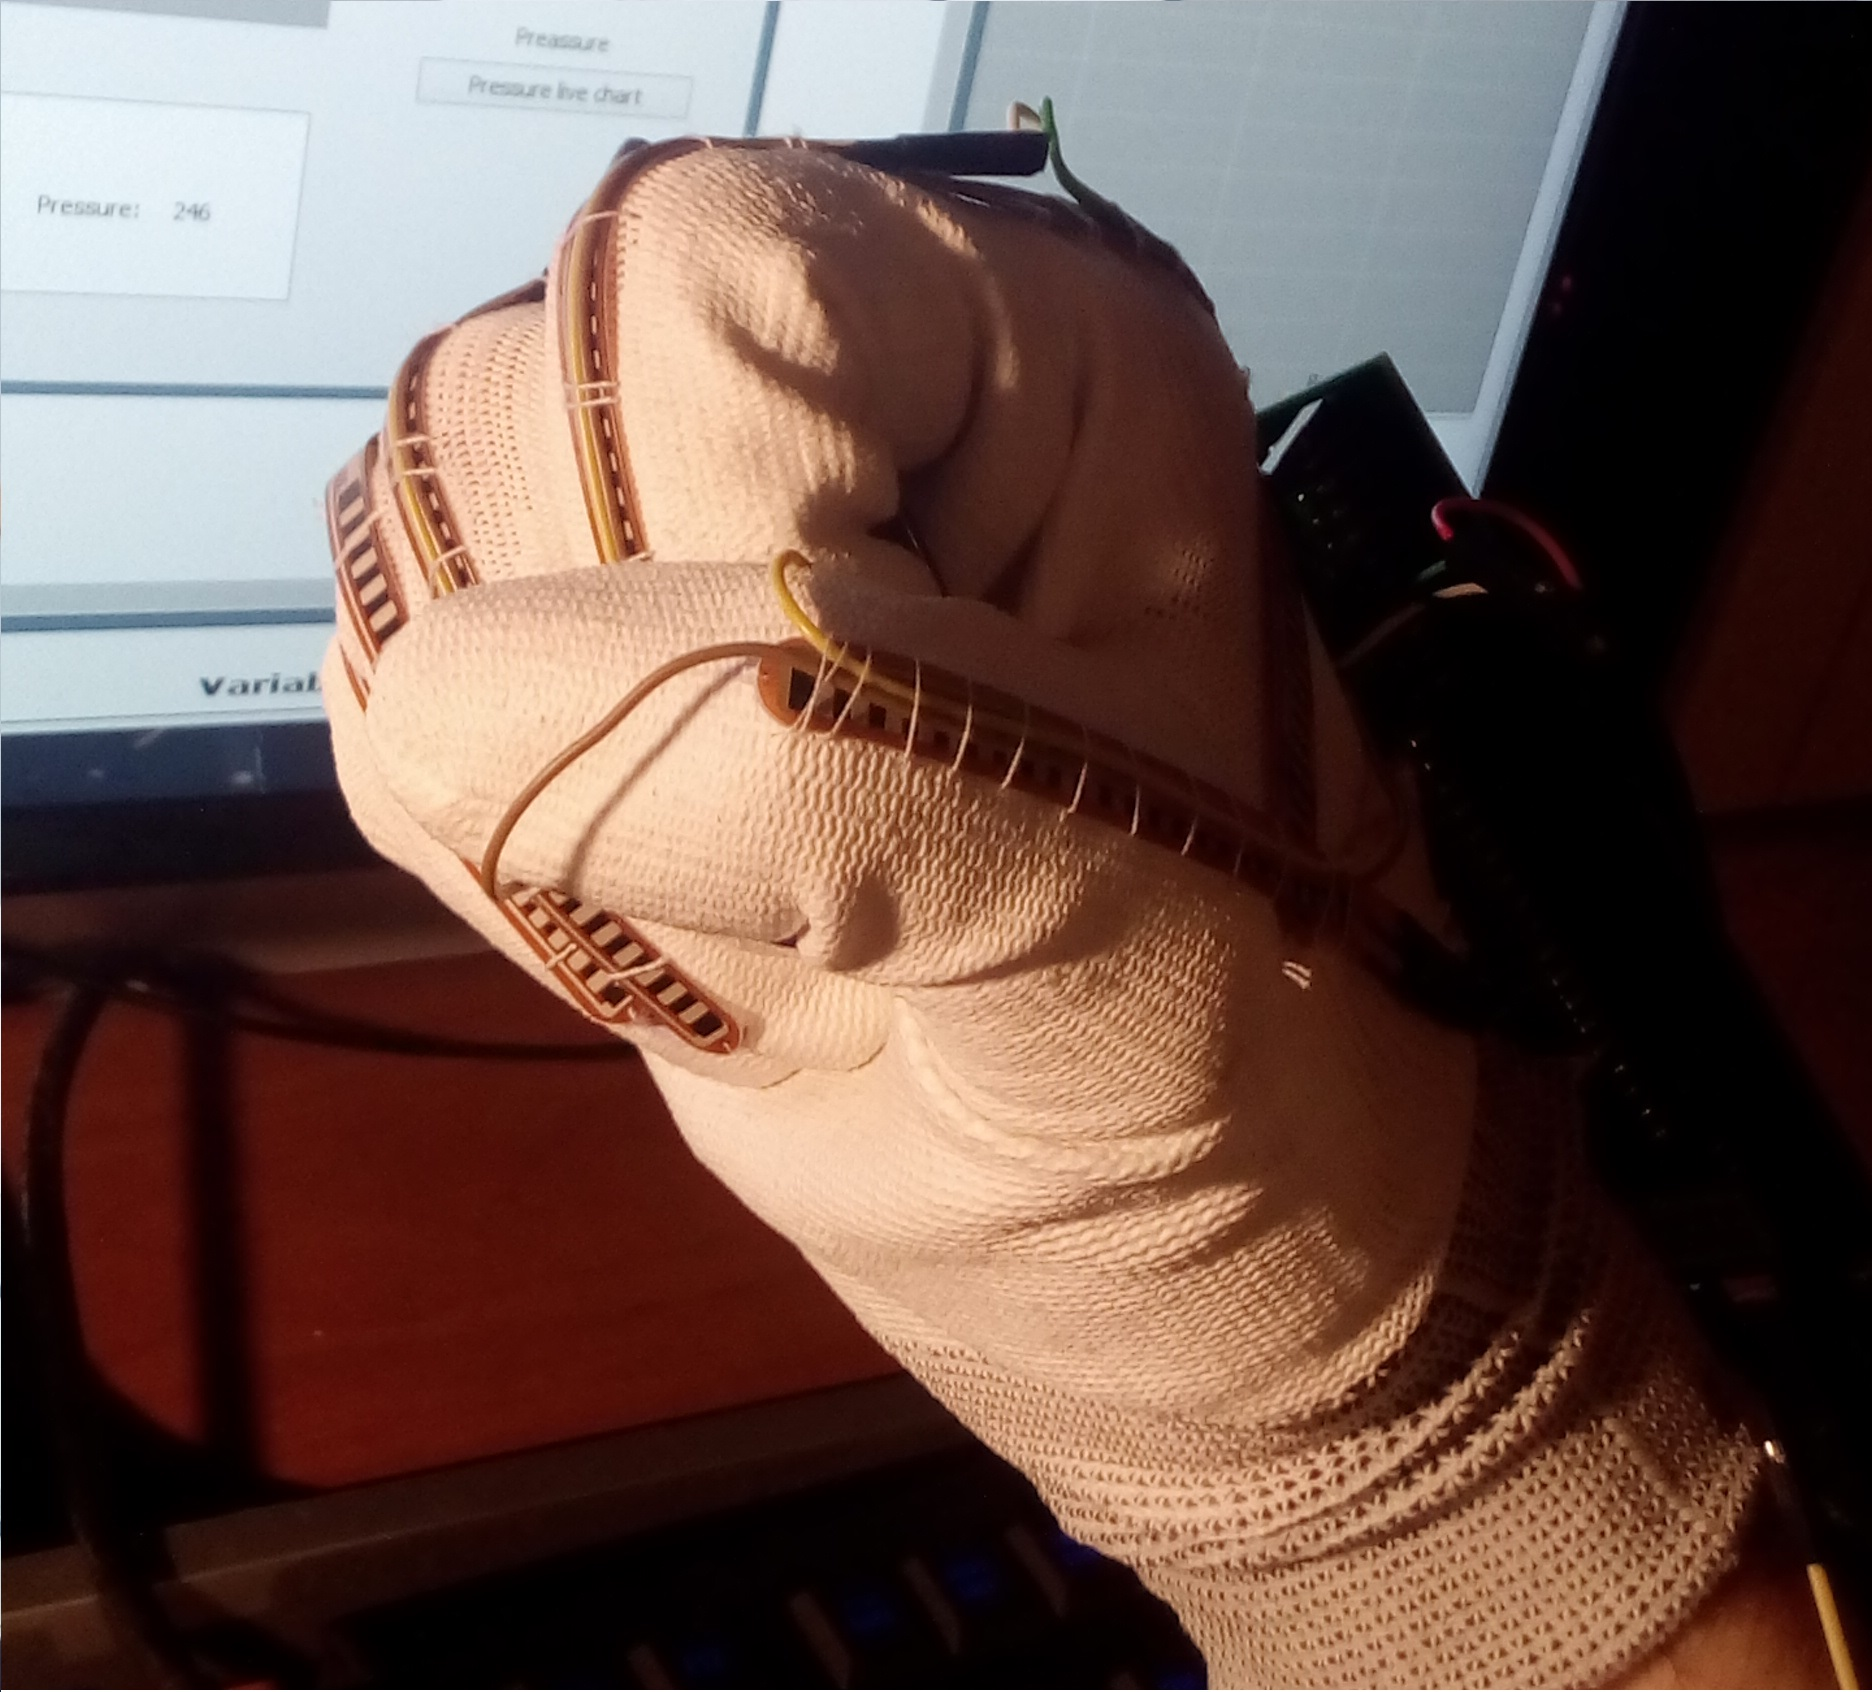
\includegraphics[width=0.9\textwidth]{./images/Fist.jpg}
     \end{subfigure}%
    \begin{subfigure}{.5\textwidth}
    \centering
      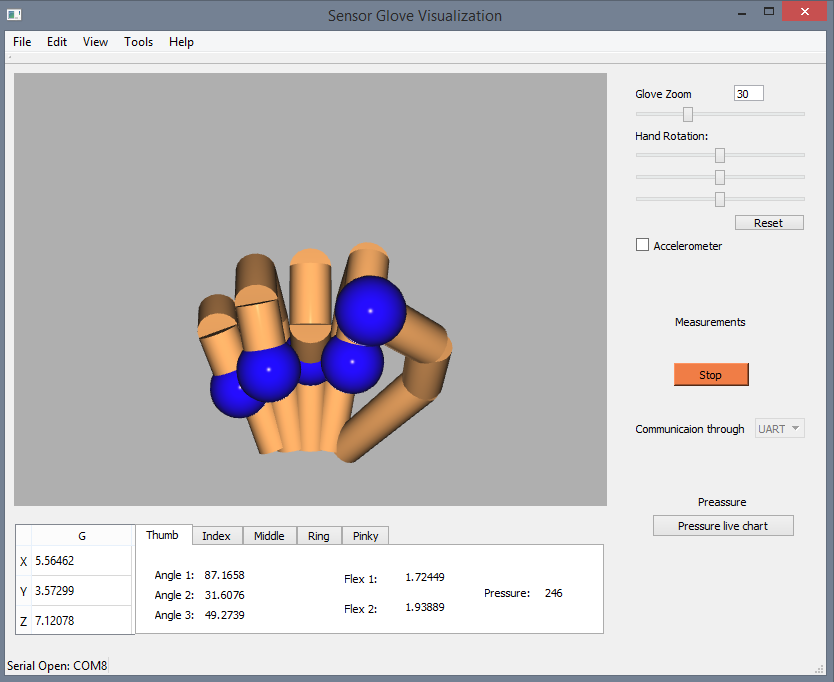
\includegraphics[width=0.9\textwidth]{./images/FistQt.png}
     \end{subfigure}
    \caption{Gest -- zaciśnięta pięść \label{fig:Fist}}
\end{figure}
\begin{figure}[!htb]
\centering
    \begin{subfigure}{.5\textwidth}
      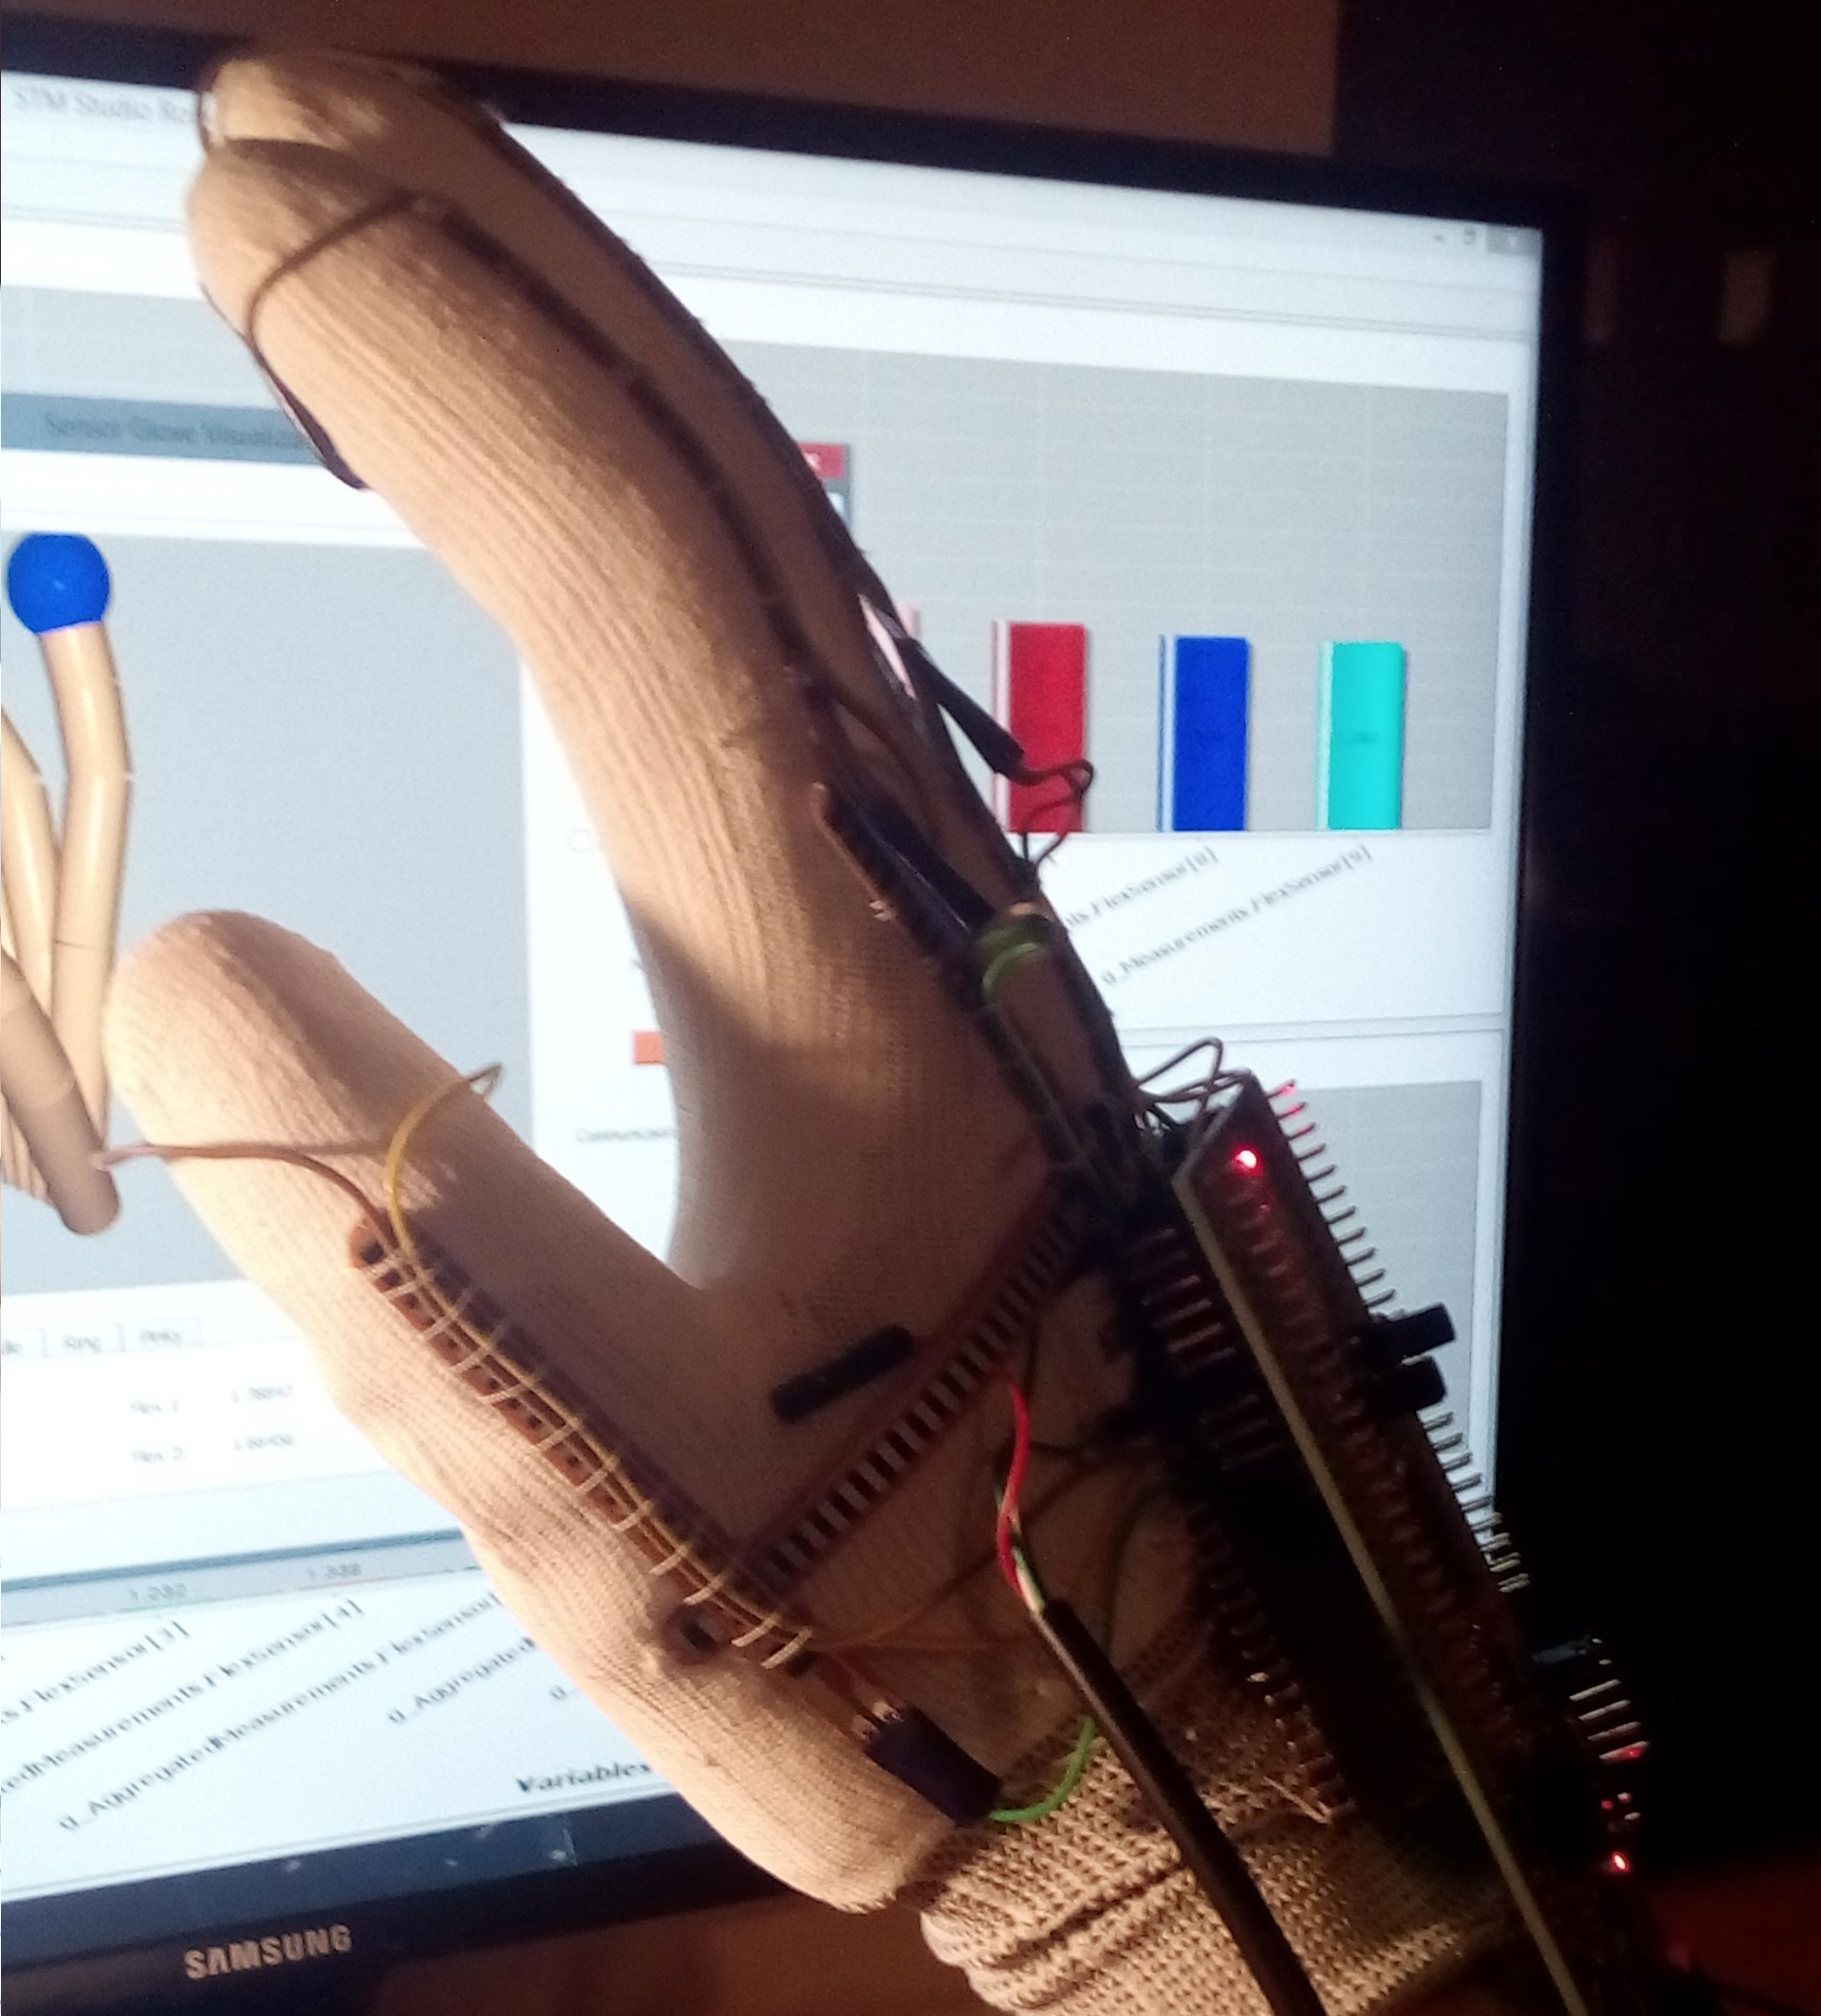
\includegraphics[width=0.9\textwidth]{./images/Palm.jpg}
     \end{subfigure}%
    \begin{subfigure}{.5\textwidth}
      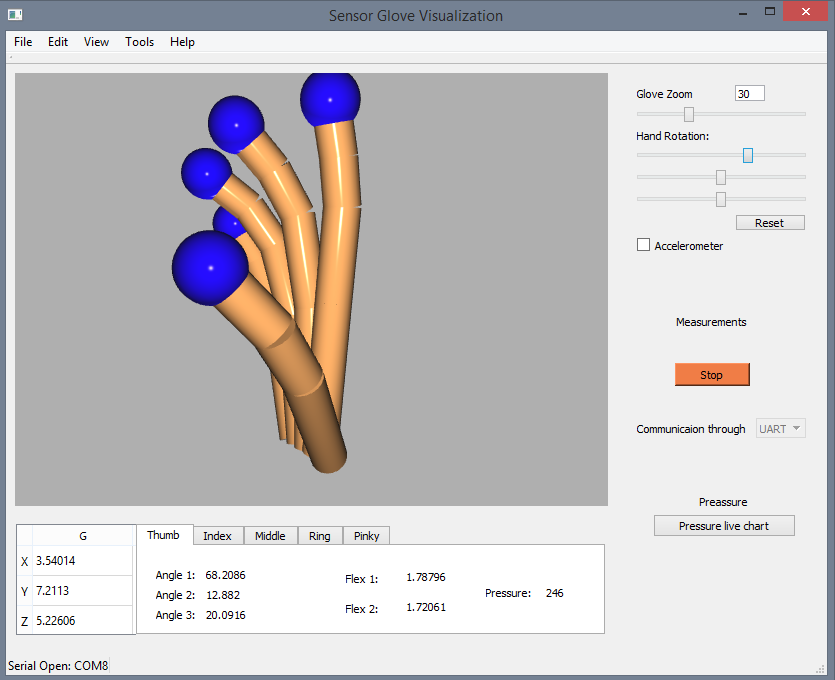
\includegraphics[width=0.9\textwidth]{./images/PalmQt.png}
     \end{subfigure}
    \caption{Gest -- otwarta dłoń \label{fig:Palm}}
\end{figure}
\begin{figure}[!htb]
\centering
    \begin{subfigure}{.5\textwidth}
      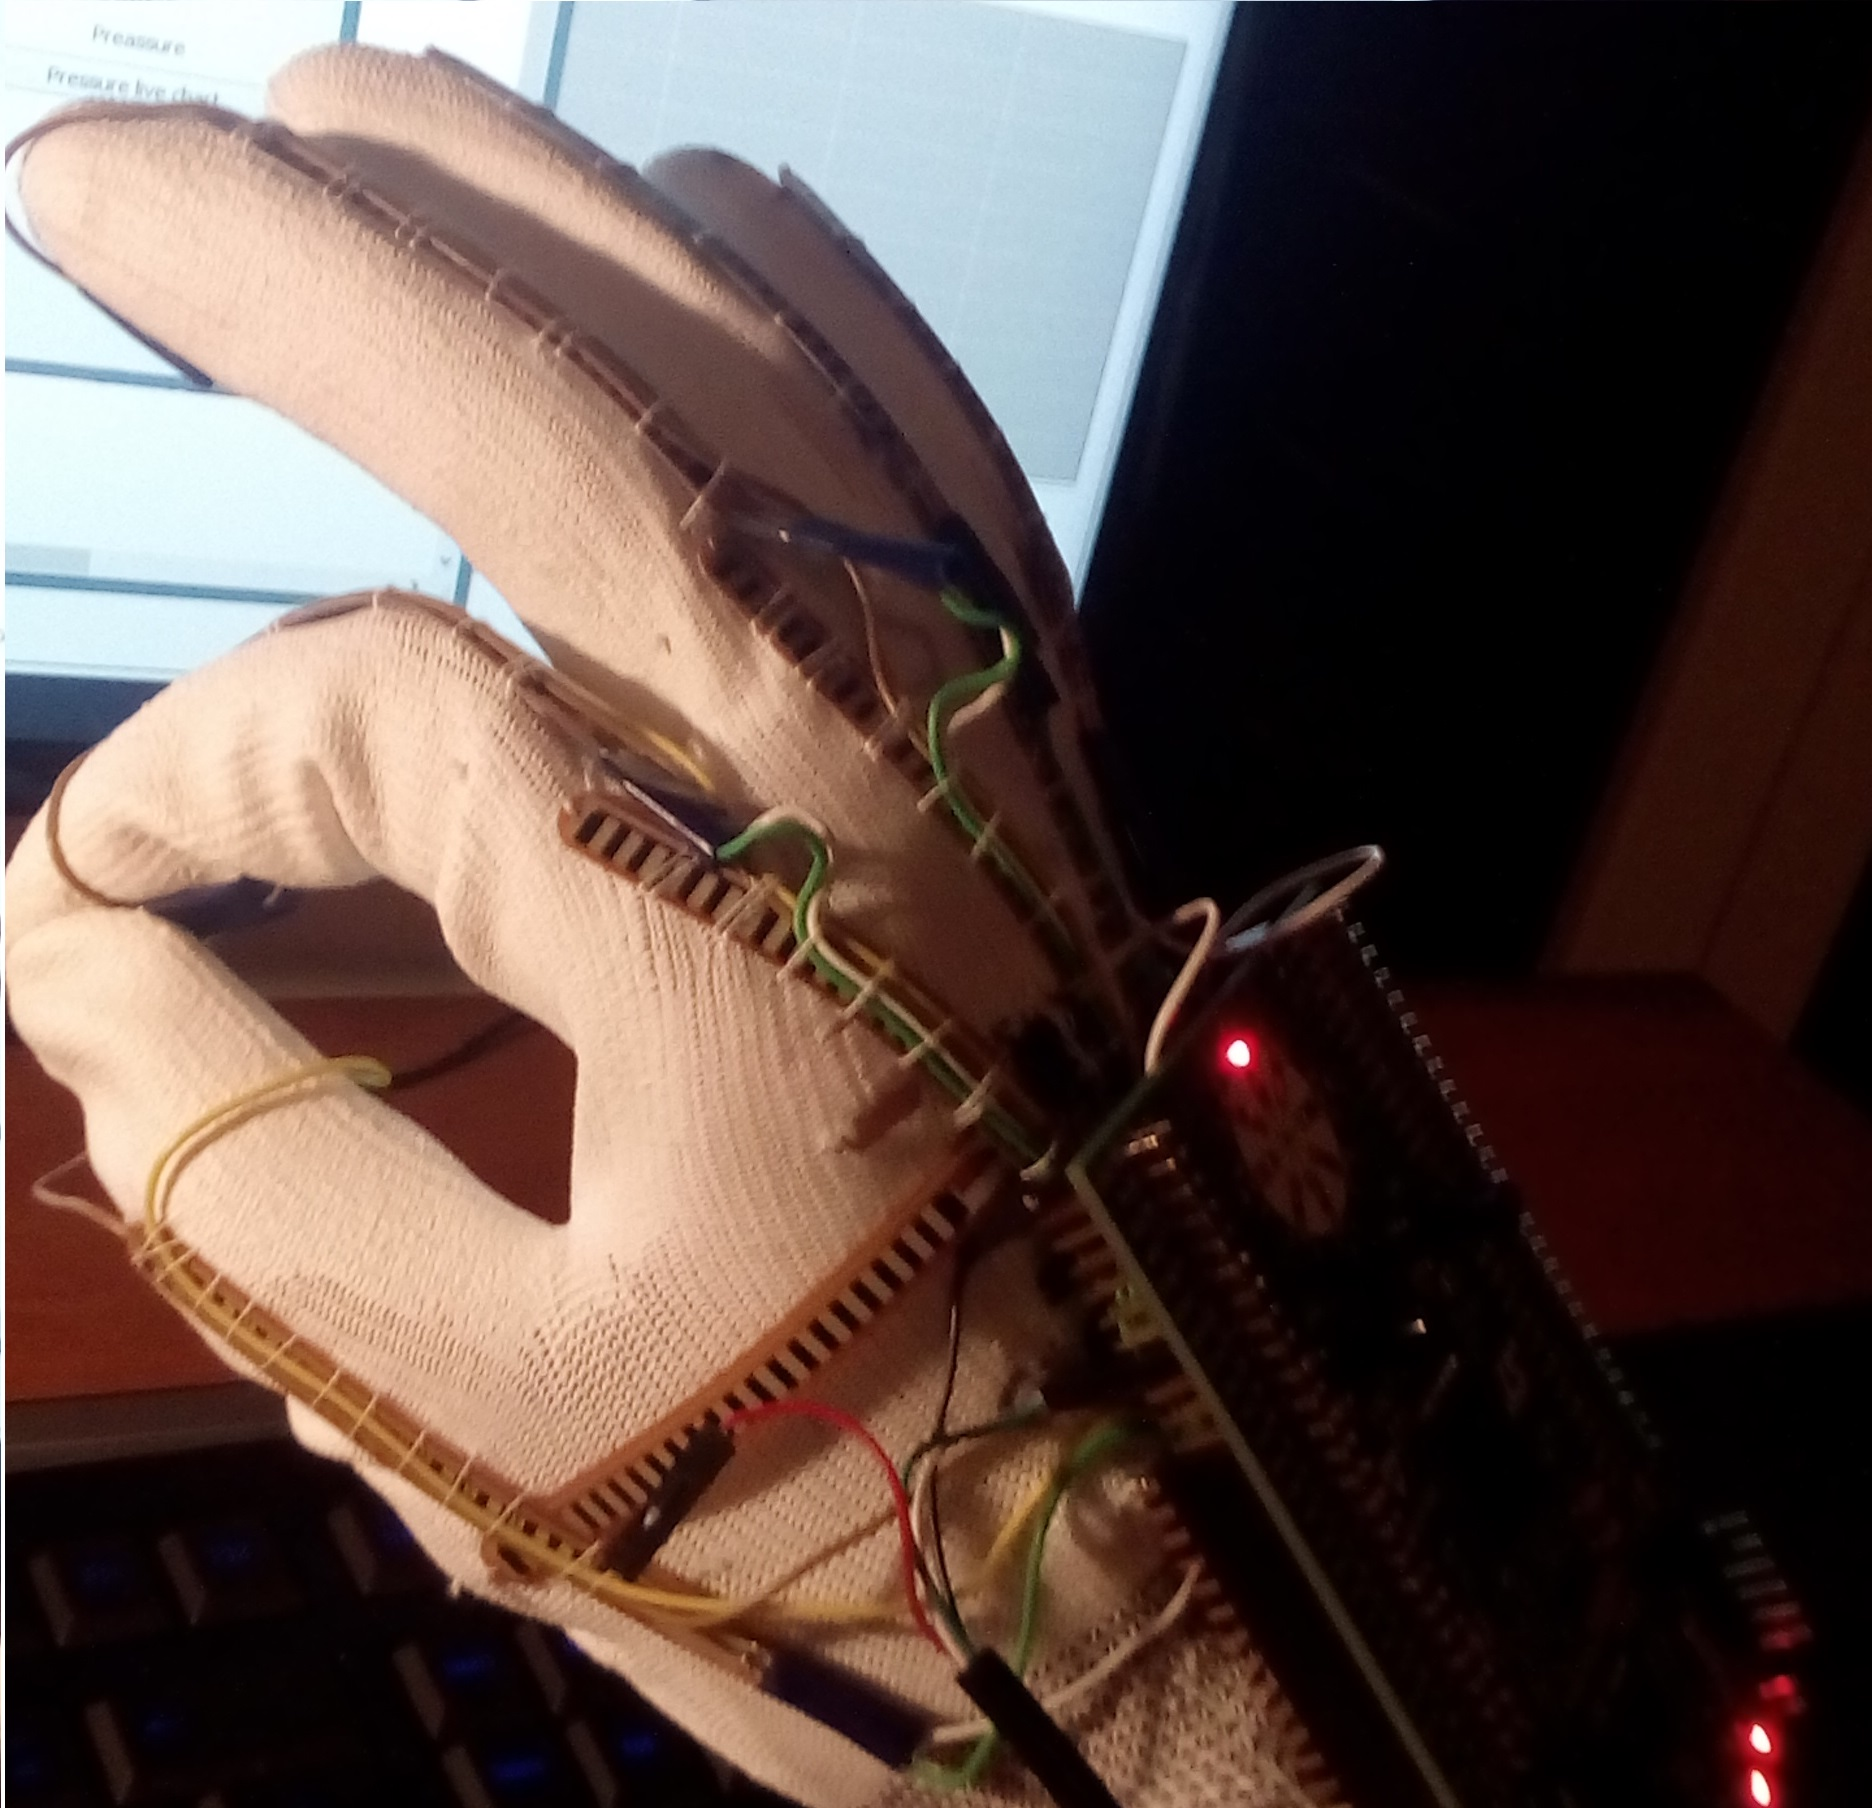
\includegraphics[width=0.9\textwidth]{./images/OK.jpg}
     \end{subfigure}%
    \begin{subfigure}{.5\textwidth}
      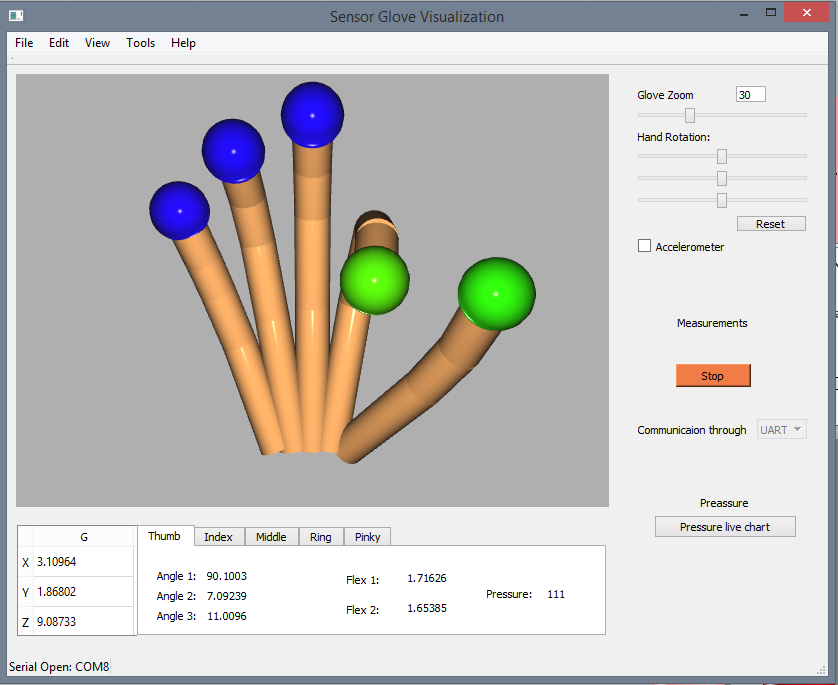
\includegraphics[width=0.9\textwidth]{./images/OKQt.png}
     \end{subfigure}
    \caption{Gest -- OK \label{fig:OK}}
\end{figure}
\begin{figure}[!htb]
\centering
    \begin{subfigure}{.5\textwidth}
      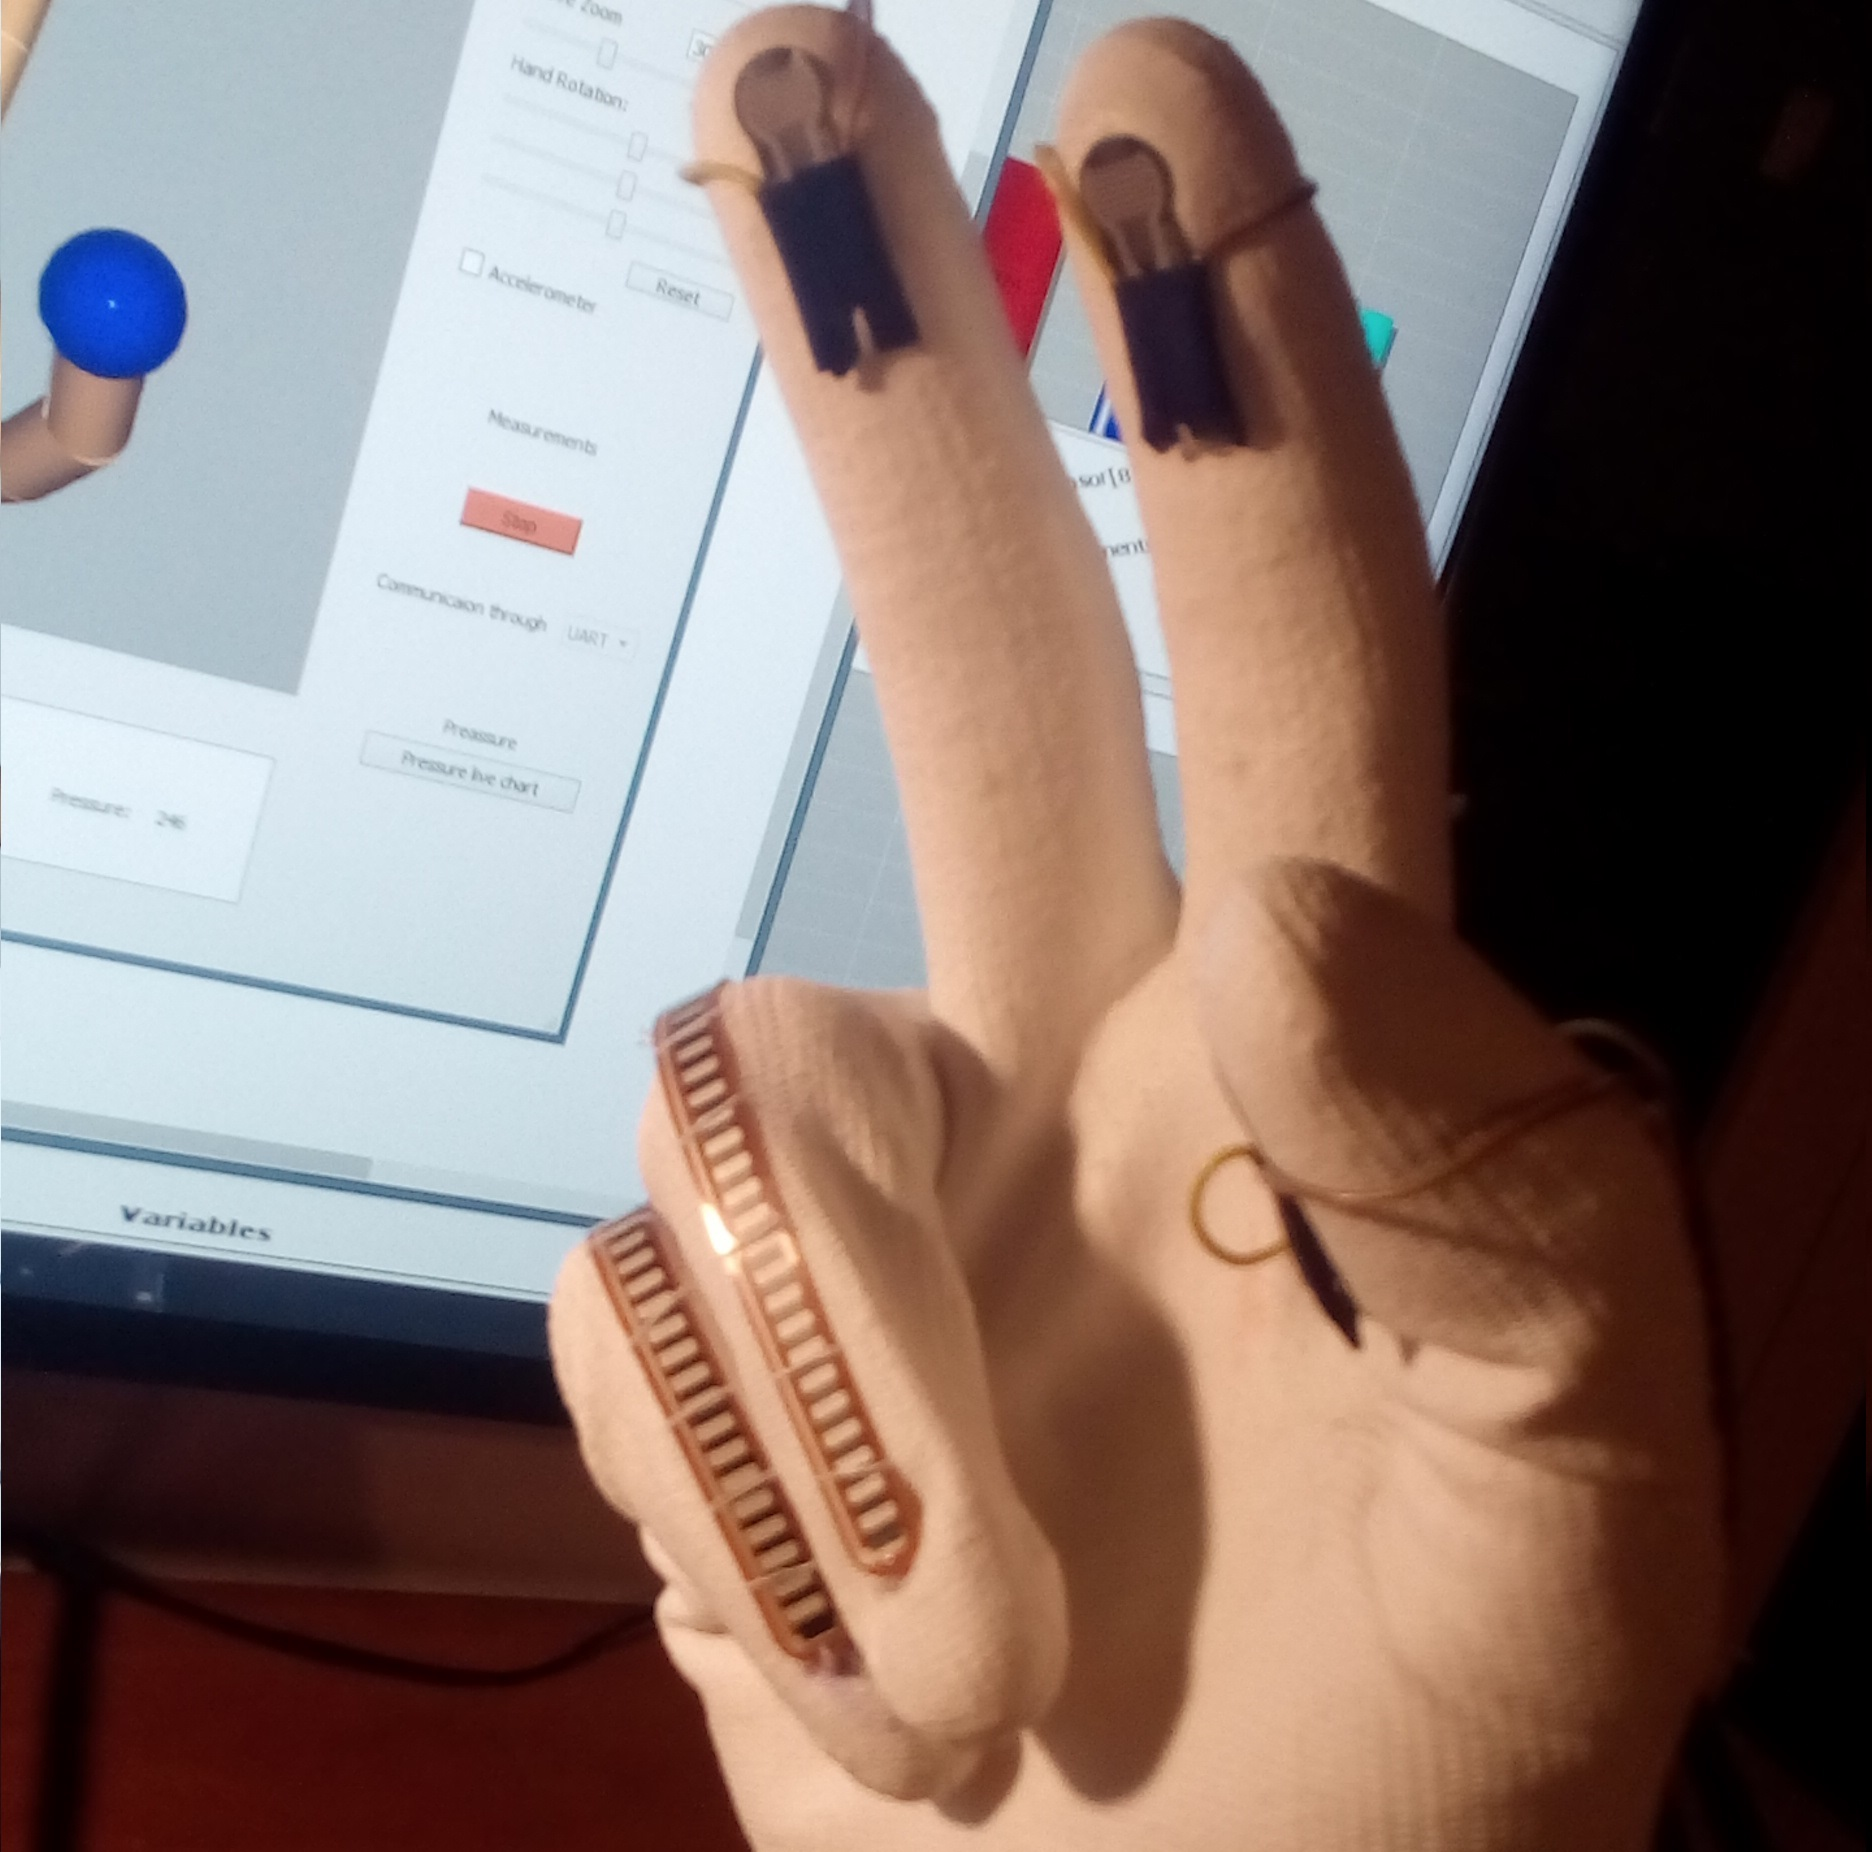
\includegraphics[width=0.9\textwidth]{./images/Peace.jpg}
     \end{subfigure}%
    \begin{subfigure}{.5\textwidth}
      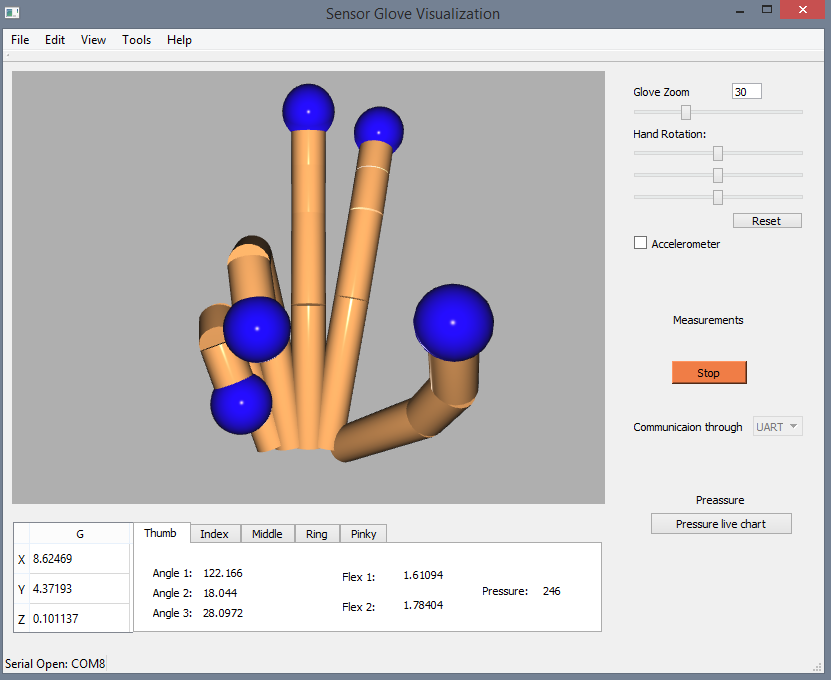
\includegraphics[width=0.9\textwidth]{./images/PeaceQt.png}
     \end{subfigure}
    \caption{Gest -- pacyfka\label{fig:Peace}}
\end{figure}
\begin{figure}[!htb]
\centering
    \begin{subfigure}{.5\textwidth}
      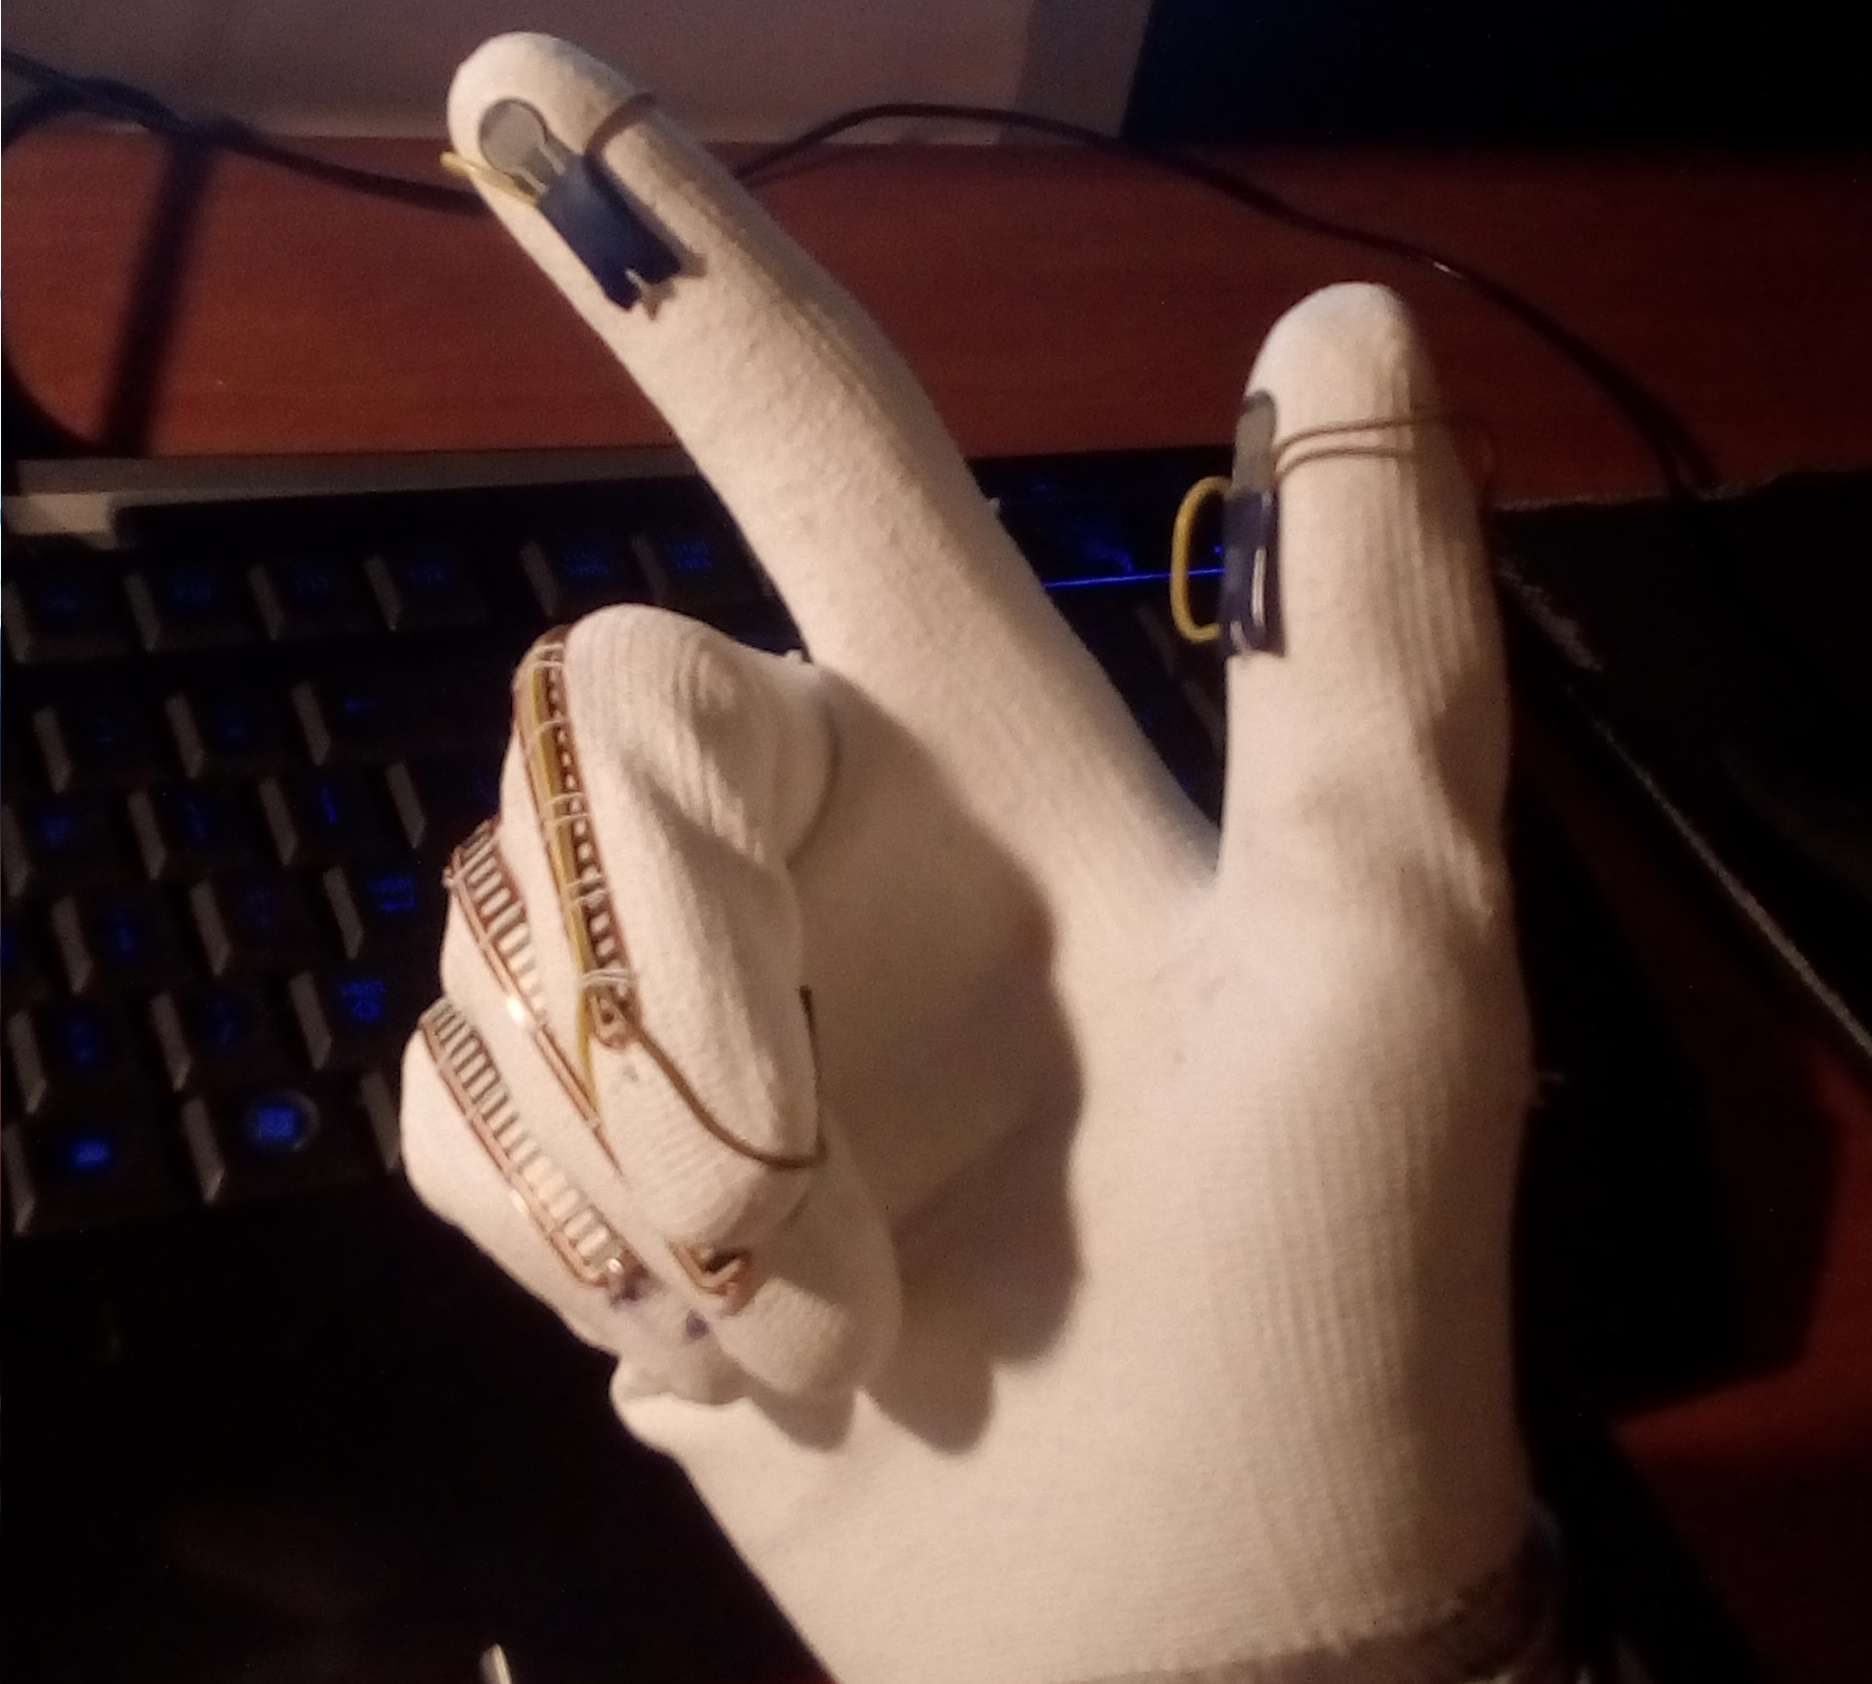
\includegraphics[width=0.9\textwidth]{./images/Point.jpg}
     \end{subfigure}%
    \begin{subfigure}{.5\textwidth}
      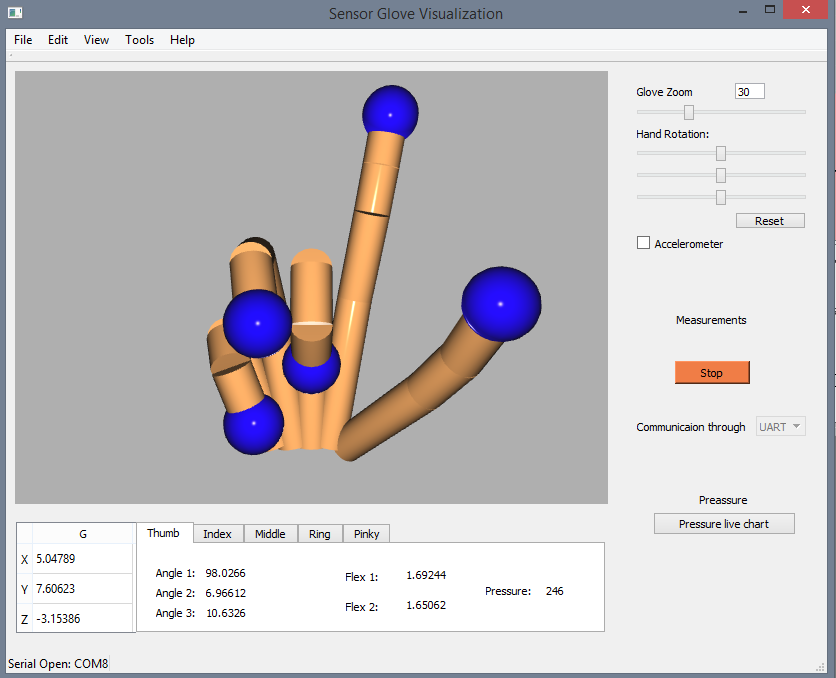
\includegraphics[width=0.9\textwidth]{./images/PointQt.png}
     \end{subfigure}
    \caption{Gest -- wskazywanie palcem \label{fig:Point}}
\end{figure}

\newpage
\section{Podsumowanie}
\subsection{Problemy podczas konstrukcji}
\begin{itemize}
\item \textit{Mała powierzchnia czujników nacisku} -- przy niektórych chwytach człowiek wykorzystuje różne części palców, np. powierzchnię boczną, a czujniki umieszczone są tylko na opuszkach
\item \textit{Problem z umieszczeniem czujnika rotacji kciuka} -- jest to złożony ruch, trudno wychwycić go jednym wąskim czujnikiem
\item \textit{Różnice w dłoniach konstruktorów} -- rękawica musi pasować do konkretnej dłoni, żeby czujniki były na odpowiednich miejscach i poprawnie zbierały pomiary
\item \textit{Mała dokładność czujników, przesuwanie się ich na rękawicy}
\item \textit{Niedoskonałość pomiarów kątów zgięcia palców} -- przy danej konstrukcji i typie czujników nie jest możliwe uzyskanie tak wysokiej dokładności, jak zakładano
\item \textit{Trudności w uzyskaniu poprawnego działania aproksymacji kątów z akcelerometru}
\item \textit{Kłopoty z interpolacją / aproksymacją} -- jest to trudne do uzyskania w C
\item \textit{Komplikacje przy zamówieniu elementów elektronicznych na katedrę} -- brak kontaktu z laborantem sprawił, że przez pewien czas nie można było uzyskać informacji, czy zamówienie zostało złożone, co poskutkowało opóźnieniem projektu
\end{itemize}
\subsection{Zmiany w założeniach projektowych}
\begin{itemize}
\item \textit{Bezprzewodowe przesyłanie danych do komputera za pomocą modułu Bluetooth} -- zrezygnowano, bo okazało się za wolne (BaudRate 9600 nie wystarcza)
\item \textit{Zamontowanie na opuszkach LEDów wizualizujących odczyty z czujników nacisku} -- zabrakło miejsca, bo czujniki trzeba było przesunąć w stosunku do wstępnego schematu, a poza tym każda dioda wymagałaby 4 kabli, co utrudniałoby ruchy dłoni
\end{itemize}
\subsection{Pomysły na rozwinięcie projektu}
\begin{itemize}
\item RPY z wielu akcelerometrów
\item Dokładniejsze pomiary i metoda interpolacji
\item Wykrywanie większej ilości gestów
\item Sterowanie robotem za pomocą gestów
\item Dodatkowe czujniki nacisku
\end{itemize}

\end{document}
